% \documentclass[review]{elsarticle}
\documentclass[utf8, babel, sor, jor, amsmath, amssymb, reprint]{elsarticle} %удалить перед отправкой
\usepackage{comment} %удалить перед отправкой
\usepackage[T2A]{fontenc} %удалить перед отправкой
\usepackage[utf8x]{inputenc} %удалить перед отправкой
\usepackage[english,russian]{babel} %удалить перед отправкой
\graphicspath{{images/}}

\usepackage{lineno,hyperref}
\usepackage{algorithm}
\usepackage{algorithmic}
\modulolinenumbers[5]

\journal{Journal of \LaTeX\ Templates}

\bibliographystyle{elsarticle-num}

\usepackage{mathrsfs}
\usepackage{amsmath}
\usepackage{amssymb}%
\usepackage{multirow}



%%%%%%%%%%%%%%%%%%%%%%%
%% Elsevier bibliography styles
%%%%%%%%%%%%%%%%%%%%%%%
%% To change the style, put a % in front of the second line of the current style and
%% remove the % from the second line of the style you would like to use.
%%%%%%%%%%%%%%%%%%%%%%%

%% Numbered
%\bibliographystyle{model1-num-names}

%% Numbered without titles
%\bibliographystyle{model1a-num-names}

%% Harvard
%\bibliographystyle{model2-names.bst}\biboptions{authoryear}

%% Vancouver numbered
%\usepackage{numcompress}\bibliographystyle{model3-num-names}

%% Vancouver name/year
%\usepackage{numcompress}\bibliographystyle{model4-names}\biboptions{authoryear}

%% APA style
%\bibliographystyle{model5-names}\biboptions{authoryear}

%% AMA style
%\usepackage{numcompress}\bibliographystyle{model6-num-names}

%% `Elsevier LaTeX' style
\bibliographystyle{elsarticle-num}
%%%%%%%%%%%%%%%%%%%%%%%


\usepackage{xcolor}
\newcommand{\todo}[1] {\textcolor{red}{#1}} %%for TODO comments
\def\l{\left\langle}
\def\r{\right\rangle}
\usepackage{mathrsfs}
\usepackage{amsmath}
\usepackage{amssymb}%

\begin{document}

\begin{frontmatter}


\title{Ground state search 2D Ising model}

\author[mainaddress, secondaryaddress]{Viacheslav Trukhin\corref{mycorrespondingauthor}}
\ead{trukhin.vo@dvfu.ru}

\author[mainaddress]{Egor Prokhorov\corref{mycorrespondingauthor}}
\ead{prokhorov.ei@dvfu.ru}

\author[mainaddress, secondaryaddress]{Aleksandr Makarov\corref{mycorrespondingauthor}}
\ead{makarov.ag@dvfu.ru}

\author[mainaddress, secondaryaddress]{Konstantin Nefedev\corref{mycorrespondingauthor}}
\ead{nefedev.kv@dvfu.ru}


\address[mainaddress]{Far Eastern Federal University, Vladivostok, Russky Island, 10 Ajax Bay, 690922, the Russian Federation}
\address[secondaryaddress]{Institute of Applied Mathematics, Far Eastern Branch, Russian Academy of Science, Vladivostok, Radio 7, 690041, the Russian Federation}

\begin{abstract}

Методом исчерпывающего перечисления были точно рассчитаны все возможные состояния модели спинового стекла Эдвардса-Андерсона и спинового льда на простой квадратной решетке 8х8 спинов. Вычислена энергия основного состояния для исследуемых образцов конечного размера. Установлено, что макроскопическое вырождение основного состояния фрустрированных спиновых систем обусловлено комбинаторикой фрустрированных плакетов, т.е. количеством вариантов размещения фрустрированных пар спинов на решетке. Алгоритм расчета энергии, спинового избытка и конфигураций основного состояния основан на определении расположения фрустраций. Зависимость спинового избытка основного состояния в модели Эдвардса-Андерсона от внешнего магнитного поля имеет дискретный (ступенчатообразный, лестничный) характер. Вычислены критические значения внешнего магнитного поля поля, при которых наблюдаются гигантские скачки энтропии. Природа больших скачков энтропии обусловлена тем, что при определенных критических значениях внешнего магнитного поля сумма нескольких конфигураций спинов с разной энергией взаимодействия и энергией Зеемана, т.е. с разным значением спинового избытка, будут обладать одинаковой полной энергией. Кратности вырождения состояний с одинаковой полной энергией суммируются.  

\end{abstract}


\begin{highlights}
	\item Наличие фрустраций в основном состоянии не обязательно приводит к макроскопическому вырождению.
	\item Энергия, энтропия и спиновый избыток основного состояния рассчитаны точно методом исчерпывающего перечисления для $8 \times 8$ спинов Изинга на квадратной решетке с открытыми граничными условиями
	\item Влияние размерного эффекта на энтропию и энергию основного состояния вычислено точно, рассчитано асимптотическое поведение энтропии
	\item Явление макроскопического вырождения основного состояния обусловлено расположением в решётке плакетов с определённой концентрацией положительных и отрицательных обменных интегралов
	\item Магнитный структурный фактор для разных конфигураций основного состояния
	\item Зависимость дисперсии магнитного момента в распределении Гиббса от энергии (количества фрустраций)
\end{highlights}


\begin{keyword}
	Ising model, GPU and CPU high performance calculations, spin ice, spin glass, statistical thermodynamics.
\end{keyword}


\end{frontmatter}

\linenumbers
\newpage
Задачи:
TO DO: \\
1. Энергия основного состояния в зависимости от размеров, асимптотическая оценка $E_{gs}(1/N)$ (есть скрипт)\\
1.2 Продолжить на большие N, показать усреднение барами. Учесть, чтобы все образцы имели одинаковое число фрустрированных плакетов (струн) \\
1.3 Проверить нормировку в статьях из таблицы, уточнить образцы \ref{tab:Egs}
1.4 Добавить в таблицу наши результаты\\
2. Поискать экспериментальные статьи по удельным Egs\\
3. Энтропия основных состояний в зависимости от размеров и асимптотика $S(1/N)$  (есть скрипт)\\
3.2 Проверить зависимость доли Ggs от всех состояний в зависимости от P+ (скорость ухождения в ноль)\\
5. Записать основные правила расстановки фрустраций (есть).\\
5.5 Разбить на главы и структурировать "правила размещения фрустрации"\\
6. Установить природу спинового избытка основного состояния \\
7. Исследовать зависимость вырождения основного состояния от количества и распределения кластеров из плакетов.\\
8. Исследовать природу макроскопического вырождения и значения спинового избытка в зависимости от распределения кластеров с возбужденными петлями по размерам. Установить какие кластеры дают наибольший вклад в вырождение. \\
10. Вычислить зависимость основного состояния от числа фрустрированных плакетов (струн) есть. Добавить нормировку и поменять представление\\
\newpage



\tableofcontents

\newpage
\section{Введение}

Без преувеличения можно сказать, что решение моделей фрустрированных систем, таких как спиновые стекла и спиновый лед, является одним из важнейших направлений исследований в статистической механике. Модель Эдвардса-Андерсона (ЕА) спинового стекла Изинга является одной из простейших моделей спиновых стекол с короткодействующими взаимодействиями \cite{edwards1975theory}. Несмотря на кажущуюся простоту, низкотемпературные свойства этой модели для 2D и более высоких размерностей до сих пор не очень хорошо изучены \cite{pal1996ground, hartmann2011ground, newman2022ground}. Модели спиновых решеток с конкурирующими ферромагнитными и антиферромагнитными взаимодействиями изучаются на протяжении множества лет \cite{binder1986spin,mezard1987spin,  lebrecht2004plaquette, valdes2012j, lebrecht2015j, fan2023searching}. 

Несмотря на многие годы интенсивных исследований, природа низкотемпературной фазы модели Изинга фрустрированных спиновых систем с ограниченным радиусом взаимодействия остается невыясненной \cite{roma2010ground, newman2023proof}. Два наиболее важных открытых вопроса касаются свойств спиновых стекол при нулевой температуре, в частности, вырождение основного состояния и природа низкоэнергетических возбуждений \cite{newman2022ground}.  

Расчет энергии, энтропии и спинового избытка основного состояния спинового стекла с заданным Гамильтонианом даже без внешнего магнитного поля является очень сложной оптимизационной задачей. В трехмерном случае задача является $NP$-трудной \cite{barahona1982computational, hartmann2002optimization}, что означает ни один известный алгоритм не может решить задачу о спиновом избытке, энергии и вырождении основного состояния за время, пропорциональное степени линейного размера системы, и считается, что такой алгоритм не может быть разработан. В настоящее время алгоритма, обладающего одновременно высокой точностью и эффективностью, не существует \cite{fan2023searching}. Свойства спиновых стекол при нулевой температуре обычно изучаются приближенными методами \cite{roma2009ground, perez2012ground}. На протяжении длительного времени разрабатываются различные приближенные подходы для решения моделей спиновых систем, но задача до сих пор остается актуальной \cite{ rybin2022hybrid, makarova2023canonical,farias2024differentiable}.  Для некоторых решеток, например, для треугольной, все же удается получить информацию об энтропийных и магнитных свойствах \cite{jurvcivsinova2024classical}. Энергия может быть рассчитана с помощью методов оптимизации \cite{hartmann2002optimization, hartmann2004new}, генетических алгоритмов \cite{holland1992adaptation}, алгоритмов отжига \cite{kirkpatrick1983optimization}, методов мультиканонического семплирования \cite{berg1994ground, shevchenko2017multicanonical}, мультиспинового кластерного метода \cite{makarova2023canonical}, параллельного отжига \cite{PhysRevB.50.16444, roma2009ground}. 

Энтропия, или вырождение основного состояния является очень важной информацией не только о низкотемпературном поведении спинового стекла (спинового льда). Задача вычисления основного состояния даже для 2D модели Эдвардса-Андерсона уже не простая задача. Даже приближенное вычисление же энтропии или кратности вырождения является намного более сложной задачей. Для ее решения разрабатывались такие методы как метод трансфер матрицы \cite{PhysRevB.22.288, cheung1983equilibrium, kolan1982ground}, баллистического поиска \cite{hartmann2000ground}, термодинамического интегрирования \cite{kirkpatrick1977frustration, binder1985monte, roma2004ground}, мультиканонического семплирования \cite{berg1994ground, shevchenko2017multicanonical}. Однако, для конечных систем, количество спинов в которых является счетным, приближенные методы навряд ли применимы. 

Модели спиновых систем на решетках представляют собой идеальную платформу для исследования сложных магнитных основных состояний с возбуждениями, что чрезвычайно важно для физики конденсированного состояния и материаловедения \cite{lacroix2011introduction}. В т.ч. вычисление значений критических полей переключения между основными состояниями во внешнем магнитном поле, скачков энтропии при переключениях между основными состояниями, корреляционных функций \cite{ramirez2004effect, rosas2004random, andriushchenko2019large}. 

Исследование энергетического ландшафта низкоэнергетических состояний спинового стекла \cite{biswas2023energy} является актуальной задачей. Тоже касается спинового льда. Интересный вопрос касается того, при какой относительной ''концентрации''  ферромагнитных обменных взаимодействий при $T=0$ будет наблюдаться переход между состоянием ферро\-маг\-не\-тиз\-ма и состоянием спинового стекла (также переход анти\-ферро\-маг\-не\-тик-спиновое стекло) \cite{gruzberg2001random, honecker2001universality, picco2006strong, tsomokos2011interplay, zimmer2022role}. Термодинамические свойства и фазовая диаграмма основного состояния относительно небольшого числа спинов молекулярных кластеров рассчитаны в работе \cite{dias2023ground}.

Конфигурации основного состояния, а также возбуждения в основном и низкоэнергетических состояниях спинового стекла, наряду с макроскопическим вырождением основного состояния и остаточной энтропией  при низких температурах активно исследуются в модели дальнодействующего дипольного взаимодействия \cite{makarova2021low, singh2024micromagnetic}. Поиск основных состояний спиновых стекол не только важен для понимания природы неупорядоченных магнетиков и многих других физических систем, но и полезен для решения широкого спектра сложных задач комбинаторной оптимизации в различных дисциплинах. Несмотря на десятилетия усилий, алгоритм, обладающий высокой точностью и эффективностью, до сих пор отсутствует \cite{fan2023searching}.

Оценка энергии основного состояния, а также выяснение природы его макроскопического вырождения являются открытыми множество лет. При низких температурах спиновое стекло в основном состоянии реализуется только за счет конфигураций, имеющих минимальную энергию взаимодействия, при этом ансамбль других конфигураций в распределении Гиббса не играет никакой роли. Энергии основного состояния рассчитанные различными методами в работах \cite{thouless1977solution, sherrington1975solvable, tanaka1980analytic, klein1976comparison, kirkpatrick1978infinite,  karandashev2019global, palmer1999ground, campbell2004energy, roma2009ground} имеют большой разброс.

Ниже будет показано, что данный разброс может быть связан с распределением вмороженного беспорядка связей, т.е. конкурирующих ферромагнитных и антиферромагнитных взаимодействий. 
Для конечного числа спинов, и энергия основного состояния будет зависеть очень сильно от конкретной реализации распределения $\left\lbrace J_{ij} \right\rbrace $ на решетке спинов. 

В настоящей работе мы использовали использован алгоритм исчерпывающего перечисления \cite{padalko2021parallel} для решения задачи об энергии основного состояния системы конечного числа спинов, вычисления вырождения этого состояния, распределения по спиновому избытку. Наличие точного решения, пусть и для относительно небольшого числа спинов, позволит тестировать приближенные методы. С помощью исчерпывающего перечисления мы нашли все состояния, поэтому мы смогли рассчитать свойства во внешнем магнитном поле. 



\section{Комбинаторика плакетов}

Пусть, под плакетом понимается замкнутая цепочка спинов минимальной длины \cite{lebrecht2015j}. В рассмотренных далее примерах на квадратной решётке плакетами являются элементарные квадраты, см. рисунки \ref{fig:Type1}, \ref{fig:Type2}, \ref{fig:Type3}. В модели спинового стекла Эдвардса-Андерсона плакеты можно разделить на три возможных типа. 

Если $P_+$ есть относительное количество ферромагнитных ($J_{ij}=+1$) обменных интегралов, тогда к первому типу, см. рис. \ref{fig:Type1}, относятся плакеты, в которых $P_+=0.5$. Для второго типа, рис. \ref{fig:Type2}, $P_+=0.75$ или $P_+=0.25$. Для третьего типа, рис. \ref{fig:Type3}, $P_+=1.0$ или $P_+=0.0$. Прямым и зубчатым линиям на рисунках соответствуют ферромагнитные и антиферромагнитные связи, соответственно. Белые и чёрные кружки на рисунках соответствуют спинам вверх и вниз в одной из конфигураций основного состояния.


\begin{figure}[H]
	\centering
	\begin{minipage}{0.3\textwidth}
		\centering
		\resizebox{45px}{45px}{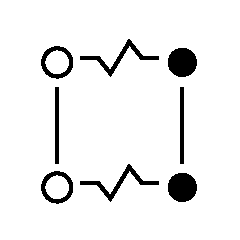
\includegraphics{pictures/Type1_1.eps}}
		\hspace{-4pt} 
		\resizebox{45px}{45px}{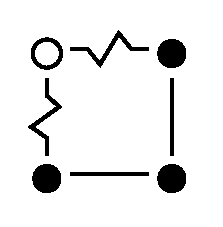
\includegraphics{pictures/Type1_2.eps}}
		\caption{Плакеты первого типа}
		\label{fig:Type1} 
	\end{minipage}
	\hspace{5pt} 
	\begin{minipage}{0.3\textwidth}
		\centering
		\resizebox{45px}{45px}{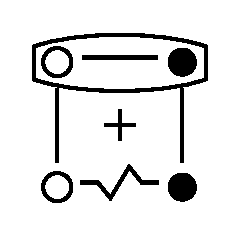
\includegraphics{pictures/Type2_1.eps}}
		\hspace{-2pt} 
		\resizebox{45px}{45px}{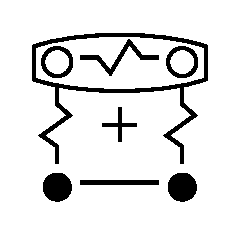
\includegraphics{pictures/Type2_2.eps}}
		\caption{Плакеты второго типа}
		\label{fig:Type2}
	\end{minipage}
	\hspace{5pt}
	\begin{minipage}{0.3\textwidth}
		\centering
		\resizebox{45px}{45px}{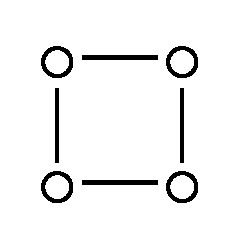
\includegraphics{pictures/Type3_1.eps}}
		\hspace{-4pt} 
		\resizebox{45px}{45px}{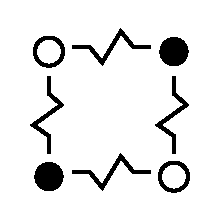
\includegraphics{pictures/Type3_2.eps}}
		\caption{Плакеты третьего типа}
		\label{fig:Type3}
	\end{minipage}
\end{figure}


В каждом из рассмотренных выше плакетов существует $2^4$ конфигураций.
Установлено, что фрустрация (возбуждение или положительная энергия обменного взаимодействия между $ij$-парой спинов) в основном состоянии обязательно появляется в плакетах второго типа, которые помечены знаком $"+"$. Причём фрустрированной парой может быть любая пара спинов.


Если система состоит из двух плакетов второго типа, например, как показано на рисунке \ref{fig:Type2_32}, то для минимизации энергии фрустрированная пара обязательно располагается на пересечении плакетов, вне зависимости от распределения обменных взаимодействий в остальной решетке. 

\begin{figure}[H]
	%\centering
	%\begin{minipage}{0.4\textwidth}
	\centering
	\begin{minipage}{0.2\textwidth}
		\centering
		(a)
		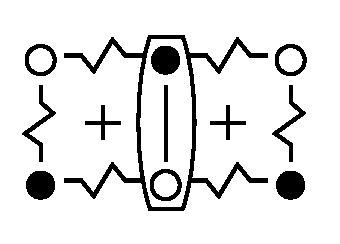
\includegraphics[width=1\textwidth]{pictures/Type2_3x2.eps}
		\label{fig:Type2_3x2}
	\end{minipage}
	\hspace{20pt}
	\begin{minipage}{0.2\textwidth}
		\centering
		(b)
		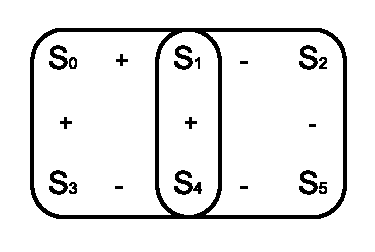
\includegraphics[width=1\textwidth]{pictures/Type2_3x2_2.eps}
		\label{fig:Type2_3x2_2}
	\end{minipage}
	\caption{Системы состоящие из двух плакетов второго типа}
	\label{fig:Type2_32}
%\end{minipage}
%\hspace{40pt}
%\begin{minipage}{0.3\textwidth}
	%\centering
	%\resizebox{100px}{70px}{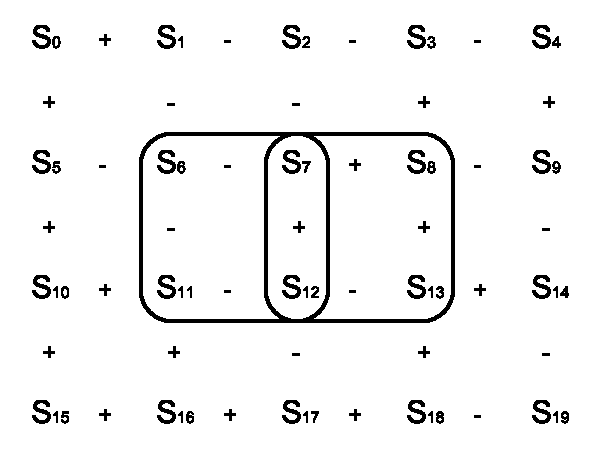
\includegraphics{pictures/Type2_5x4.eps}}
	%\caption{Система из 20 спинов с двумя плакетами 2-го типа в центре}
	%\label{fig:Type2_5x4}
%\end{minipage}
\end{figure}


Легко найти энергию, спиновый избыток и конфигурации основного состояния при известном расположении фрустрированных пар спинов. Энергия и кратность вырождения основного состояния для систем на рисунке \ref{fig:Type2_32} $E_{gs}/N=-0.83$, $g=2$. Спиновый избыток основного состояния $M_{gs}/N=0$ для системы на рисунке \ref{fig:Type2_32}(a) и $M_{gs}/N=\pm 0.33$ на рисунке \ref{fig:Type2_32}(b).

%На рисунке \eqref{fig:Type2_5x4} представлена система из двадцати спинов, в центре которой находятся два плакета 2-го типа, имеющие общую пару спинов. Исходя из предыдущего примера, данная система должна обладать одной фрустрированной парой отмеченной на рисунке. Полный перебор состояний подтверждает, что в данной системе есть два основных состояния ($E_{gs}/N=-1.45$, $M_{gs}=\pm 8$), а фрустрация действительно расположена так, как показано на рисунке \eqref{fig:Type2_5x4}.

На рисунках \ref{fig:4x4.1} в центре решетки находится плакет 2-го типа, содержащий фрустрацию. Размещение фрустрации в плакете не 2-го типа приводит к возникновению еще одного возбуждения в нем. В данном примере существует 8 основных состояний ($E_{gs}/N=-1.25$, $g=8$, $M_{gs}/N=\pm 0.25$ - рисунок \ref{fig:4x4.1} (a), $M_{gs}/N=\pm 0.25$ - рисунки \ref{fig:4x4.1} (a,b), $M_{gs}/N=\pm 0.08$ - рисунок \ref{fig:4x4.1} (c), $M_{gs}/N=\pm 0.08$ - рисунок \ref{fig:4x4.1} (d),). Спиновый избыток основного состояния обусловлен соотношением количества ферромагнитных и антиферромагнитных связей. Фрустрации могут изменять это соотношение, потому что фрустрированная антиферромагнитная связь приведет к ферромагнитному упорядочению в паре спинов, и наоборот.

\begin{figure}[H]
	\begin{minipage}[h]{0.2\linewidth}
		\centering(a)
		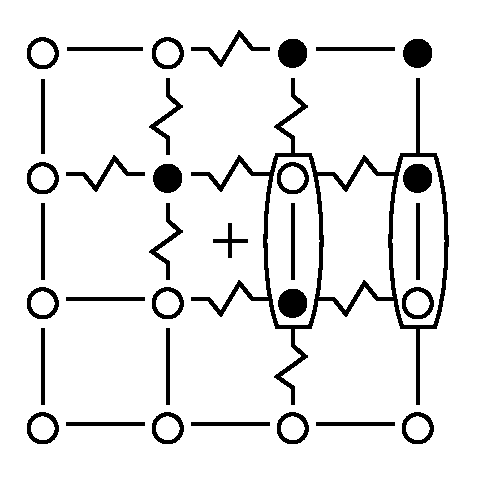
\includegraphics[width=1\linewidth]{pictures/Cl1_Type2_gs1.eps}
	\end{minipage}
	\hfill
	\begin{minipage}[h]{0.2\linewidth}
		\centering(b)
		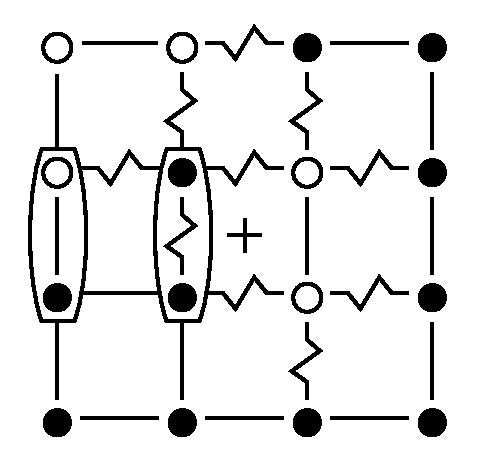
\includegraphics[width=1\linewidth]{pictures/Cl1_Type2_gs2.eps}
	\end{minipage}
	\hfill
	\begin{minipage}[h]{0.2\linewidth}
		\centering(c)
		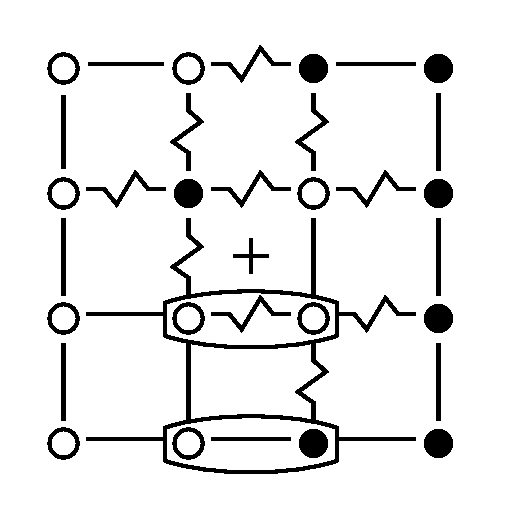
\includegraphics[width=1\linewidth]{pictures/Cl1_Type2_gs3.eps}
	\end{minipage}
	\hfill
	\begin{minipage}[h]{0.2\linewidth}
		\centering(d)
		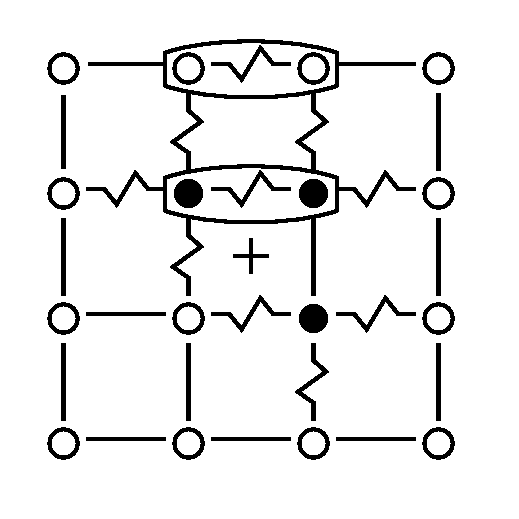
\includegraphics[width=1\linewidth]{pictures/Cl1_Type2_gs4.eps}
	\end{minipage}
	\caption{Основные состояния системы (a, b, c, d). Фрустрированные пары спинов обведены.}
	\label{fig:4x4.1}
	
\end{figure}

Для примера на рисунке \ref{fig:4x7}, $E_{gs}/N=-1.18$, $M_{gs}/N=0$, существует только два основных состояния $g=2$. При этом имеется три фрустрированные пары. Таким образом, наличие фрустраций в основном состоянии не всегда приводит к макроскопическому вырождению. 

\begin{figure}[H]
	\centering
	\resizebox{150px}{75px}{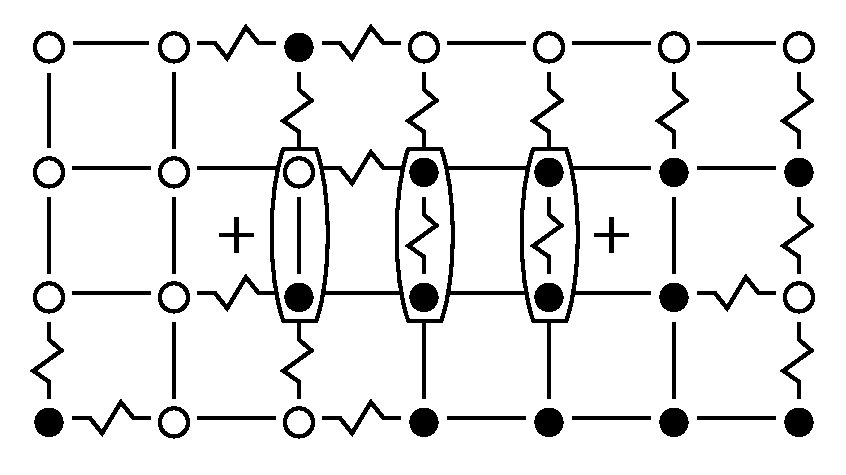
\includegraphics{pictures/Cl7x4_Type2.eps}}
	\caption{Основное состояние решетки с двумя плакетами второго типа}
	\label{fig:4x7}
\end{figure}

На рисунке \ref{fig:5x5.22F} приведен пример ($E_{gs}/N=-1.44$, $g=4$, $M_{gs}/N=\pm 0.11$ для рисунка \ref{fig:4x7} (a) и $M_{gs}=\pm 0.04$ для \ref{fig:4x7} (b)), когда два плакета 2-го типа имеют один общий спин. Несмотря на уменьшение количества фрустрированных пар, по сравнению с предыдущим примером, наблюдается увеличение вырождения основного состояния. Комбинаторика возникает по причине того, что ???? фрустрации в основном состоянии будут находиться между плакетами 2-го типа. Разница лишь в том, что один спин будет входить сразу в две фрустрированные пары.

\begin{figure}[H]
	\centering
	\begin{minipage}[h]{0.25\linewidth}
		\centering(a)
		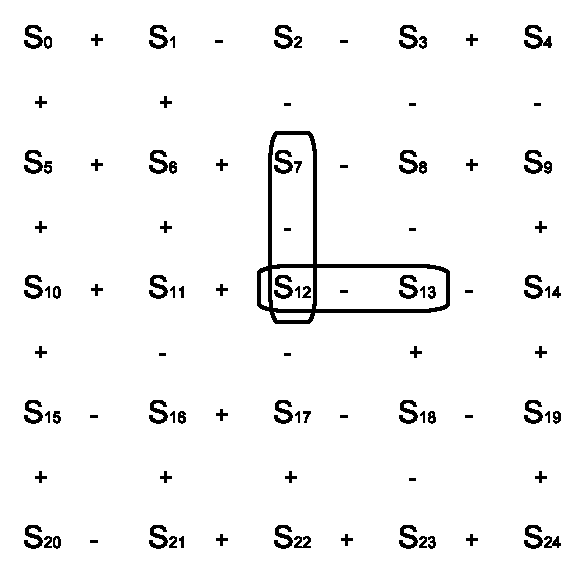
\includegraphics[width=1\linewidth]{pictures/Cl5x5_Type2_gs1.eps}
	\end{minipage}
	\hspace{15pt}
	\begin{minipage}[h]{0.25\linewidth}
		\centering(b)
		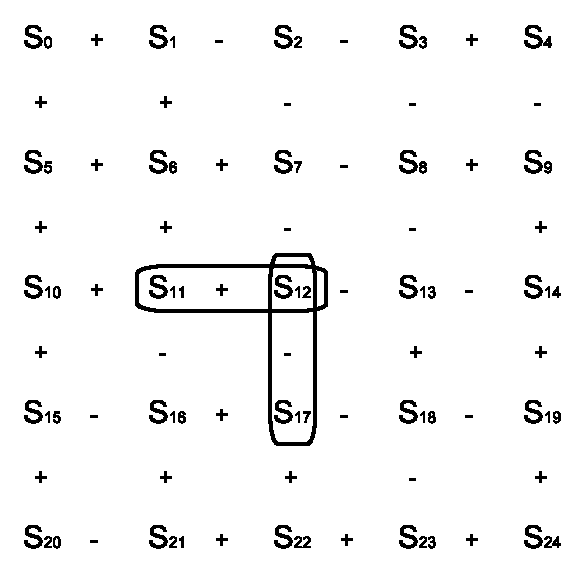
\includegraphics[width=1\linewidth]{pictures/Cl5x5_Type2_gs2.eps}
	\end{minipage}
	\caption{Основные состояния решетки с двумя плакетами второго типа}
	\label{fig:5x5.22F}
\end{figure}

На основе рассмотренных примеров можно сделать несколько выводов:

1. Плакеты 2-го типа являются единственной причиной возникновения фрустраций в основном состоянии.

2. В основном состоянии фрустрации расположены между плакетами 2-го типа или между плакетом и краем решётки в зависимости от расстояний.

3. Макроскопическое вырождение основного состояния подразумевает альтернативные варианты размещения фрустраций.


\section{Природа вырождения основного состояния}

Можно вычислить все основные состояния путём попарного комбинирования плакетов 2-го типа.
Рассмотрим работу алгоритма на примере решётки состоящей из 64 спинов \ref{fig:12PS_cell64_J72_5} (a).

\begin{figure}[H]
	\centering
	\begin{minipage}[h]{0.3\linewidth}
		\centering(a)
		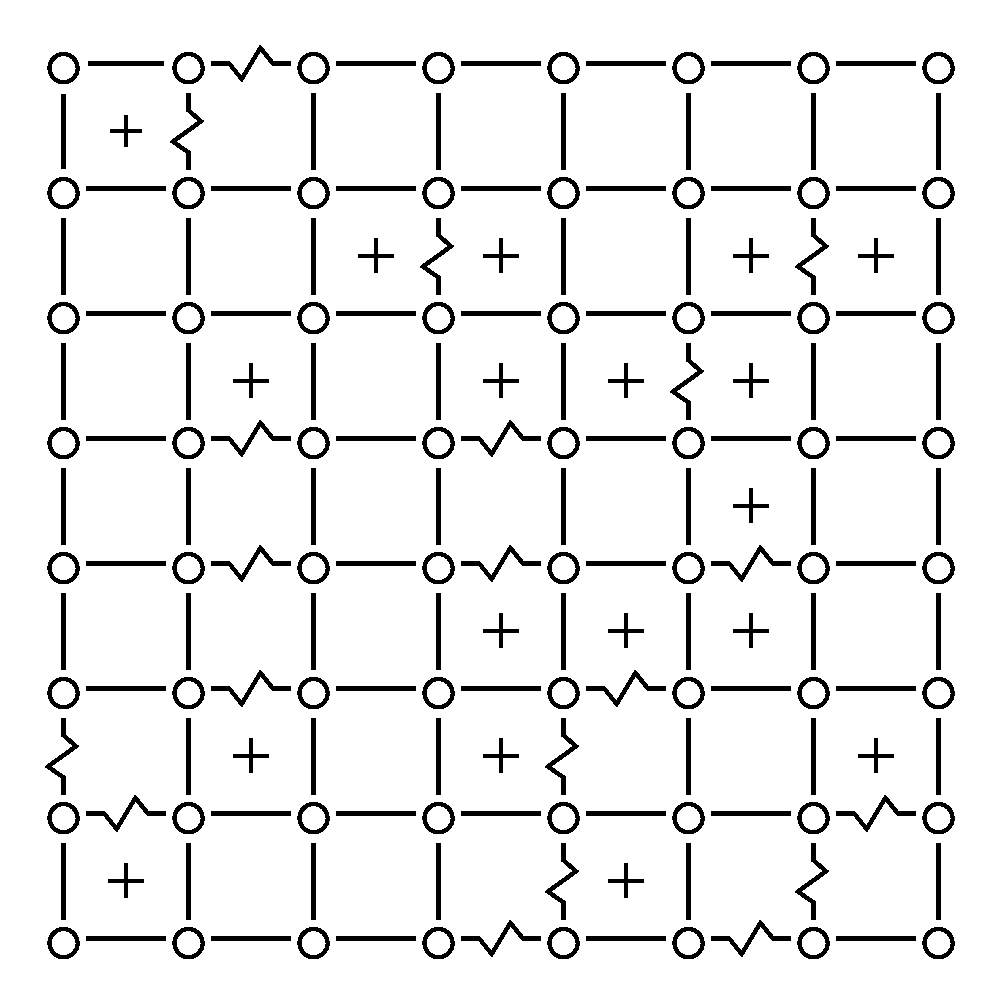
\includegraphics[width=1\linewidth]{pictures/cell64_J72_5.eps}
	\end{minipage}
	\hspace{10pt}
	\begin{minipage}[h]{0.3\linewidth}
		\centering(b)
		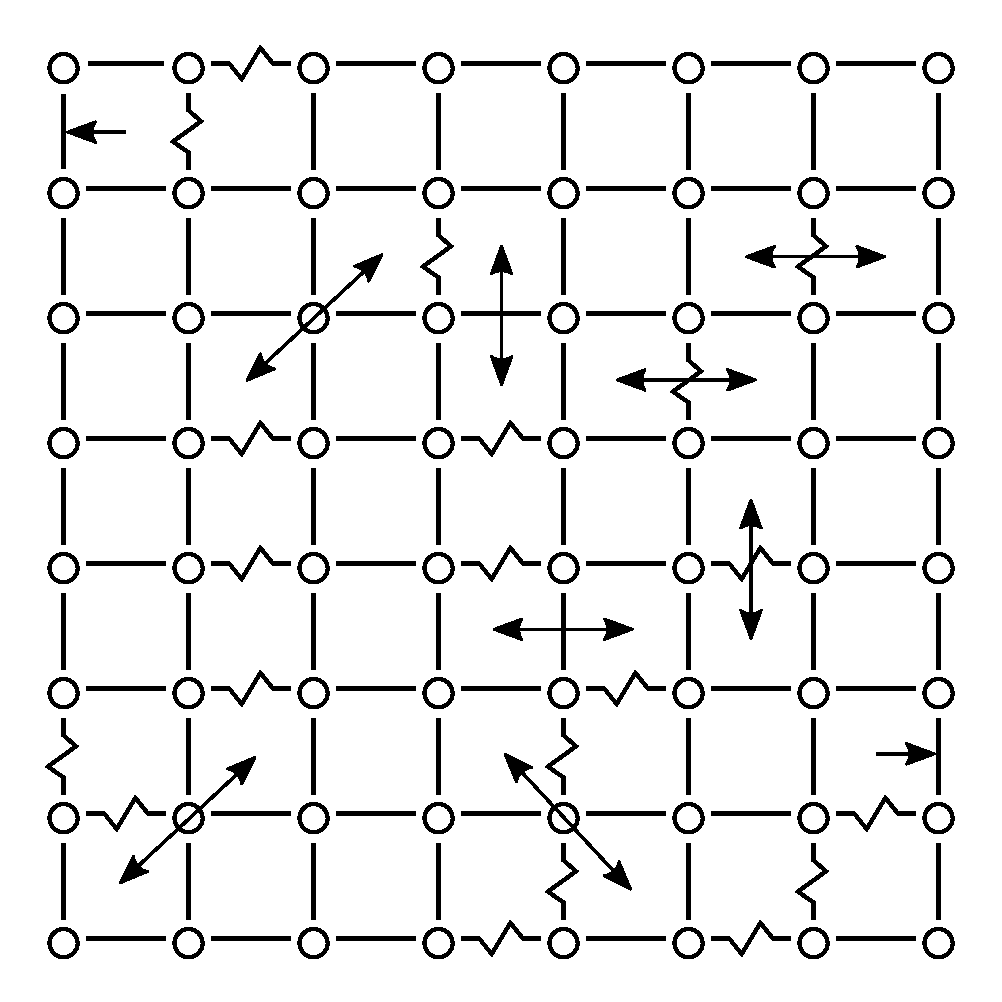
\includegraphics[width=1\linewidth]{pictures/1PS_cell64_J72_5.eps}
	\end{minipage}
	\hspace{10pt}
	\begin{minipage}[h]{0.3\linewidth}
		\centering(c)
		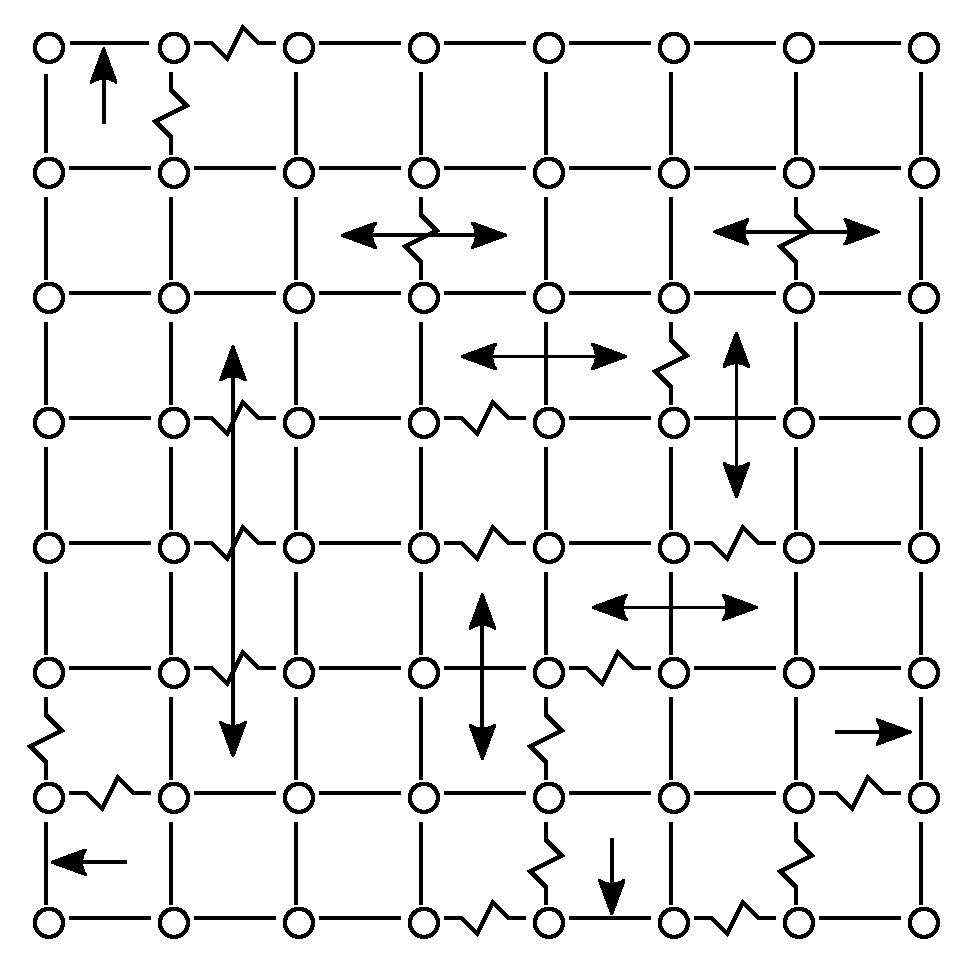
\includegraphics[width=1\linewidth]{pictures/2PS_cell64_J72_5.eps}
	\end{minipage}
	\caption{(a) - пример решетки 64 спина, (b,c) - комбинации плакетов 2-го типа, обладающих минимальным числом фрустраций}
	\label{fig:12PS_cell64_J72_5}
\end{figure}


Сначала каждому плакету присваиваются координаты $x$ и $y$. Далее происходит комбинирование разбиений плакетов второго типа по парам. Рассматриваются случаи, когда фрустрации возникают между каждой парой плакетов и когда размещение возбуждений происходит между плакетом и краем решётки. Число фрустраций между $i,j$-той парой плакетов определяется как $\left|x_i-x_j\right|+\left|y_i-y_j\right|$,  число фрустраций, возникающее от плакета 2-го типа до ближайшего края решетки определяется как $R_{ij}+1$, где i - номер плакета 2-го типа, j - номер ближайшего плакета находящегося на краю решётки, $R_{ij}$ - расстояние между ними. После перебора всех пар плакетов 2-го типа рассматриваются комбинации, которые по подсчётам обладают минимальным числом фрустраций. Две из них представлены на рисунке \ref{fig:12PS_cell64_J72_5} (b,c).

На основании полученных комбинаций пары спинов, находящиеся между плакетами, отмечаются как фрустрированные (рис. \ref{fig:12F_cell64_J72_5}).

\begin{figure}[H]
	\centering
	\begin{minipage}[h]{0.3\linewidth}
		\centering(a)
		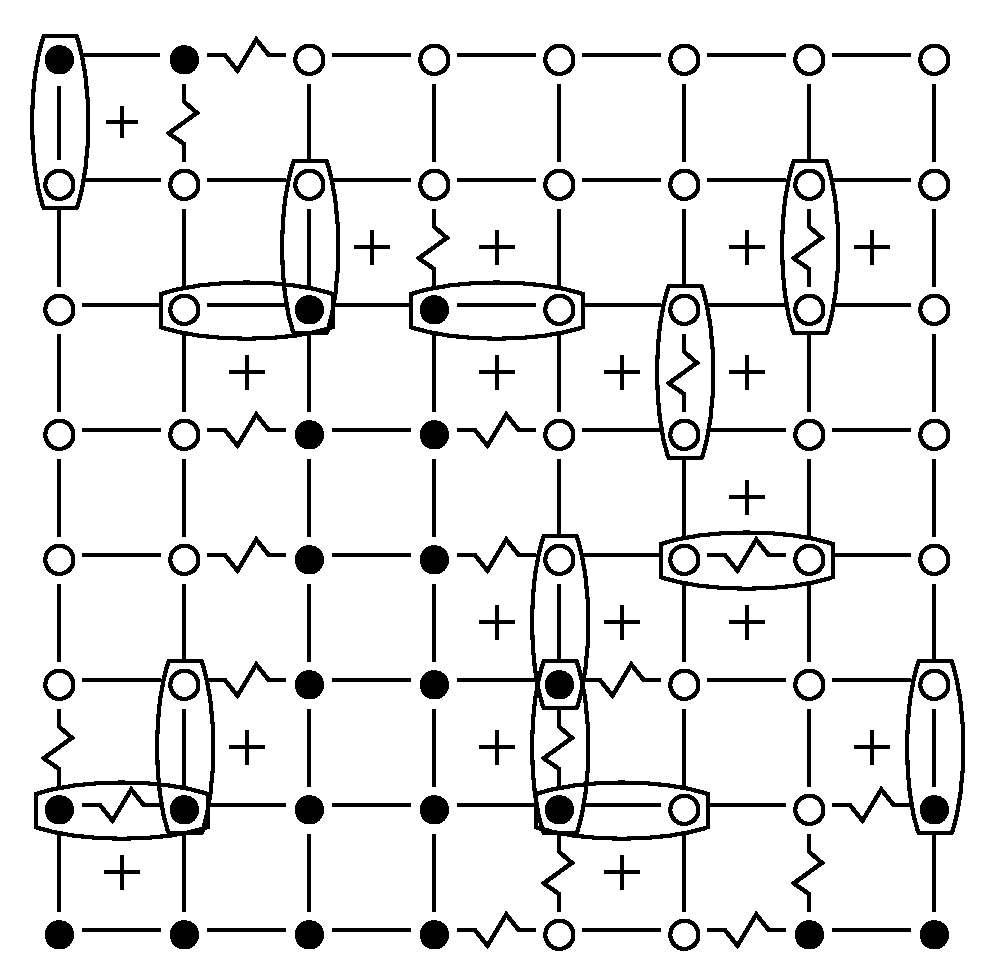
\includegraphics[width=1\linewidth]{pictures/1Conf_cell64_J72_5.eps}
	\end{minipage}
	\hspace{15pt}
	\begin{minipage}[h]{0.3\linewidth}
		\centering(b)
		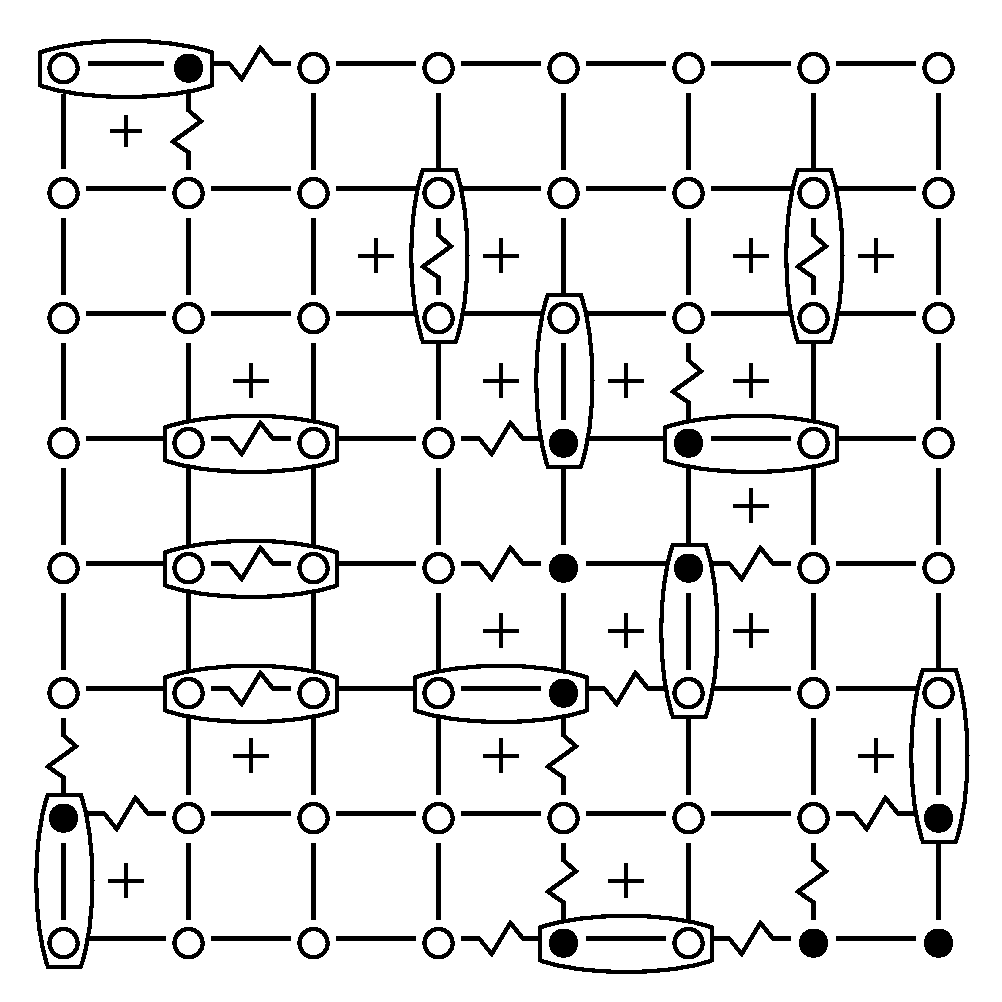
\includegraphics[width=1\linewidth]{pictures/2Conf_cell64_J72_5.eps}
	\end{minipage}
	\caption{Основные состояния решетки \ref{fig:12PS_cell64_J72_5} (a)}
	\label{fig:12F_cell64_J72_5}
\end{figure}

Всего для данной решётки было получено $g=124$ основных состояния с энергией $E_{gs}/N=-1.34$ и спиновым избытком $M_{gs}/N$ от $\pm 0.28$ до $\pm 0.66$. Данное решение полностью совпадает с результатами, полученными с помощью алгоритма \ref{alg:addititional_algorithm}.

Таким образом, высокая кратность вырождения основного состояния обусловлена несколькими причинами:

1. Различные комбинации плакетов 2-го типа могут давать одинаковое количество фрустраций, как показано в предыдущем примере на рисунках \ref{fig:12PS_cell64_J72_5} (b,c).

2. Может существовать несколько вариантов размещения фрустраций между плакетами, если их координаты $x,y$ различаются (рис. \ref{fig:5x5.22F}).

3. Выбор граничных условий может влиять на вырождение. Например в случает размещения фрустрированного плакета рядом с двумя границами приводит к увеличению вариантов размещения фрустраций (рис. \ref{fig:4x4.1}).



\section{Решение исчерпывающим перечислением}

Модель спинового стекла Эдвардса-Андерсона представляет собой плоскую решетку Изинга:

\begin{equation}
	E = -\sum J_{ij} S_i S_j + h \sum S_i.
	\label{eq:ising_energy}
\end{equation}
Это приводит к конкурирующим антиферромагнитным (при $J_{ij}=-1$) и ферромагнитным (при $J_{ij}=+1$) взаимодействиям. В нашей модели энергия обменного взаимодействия не зависит от расстояния между взаимодействующими спинами. Однако, знакопеременный характер обменных интегралов $J_{ij}$ может быть связан с искажениями в размещении взаимодействующих атомов на решетке, осцилляциями электронной плотности.

Рассмотрим одномерную цепочку из трёх спинов ($L=3$), взаимодействующих ферромагнитно.  В этом случае $J_{ij}=+1$.  Обозначим $\beta = (kT)^{-1}$.  Статистическая сумма принимает вид:

\begin{equation}
	Z_3 = e^{3\beta - 3\beta h} + 3e^{\beta - h - \beta} + 3e^{\beta h - \beta} + e^{3\beta + 3\beta h}.
	\label{eq:stat_3}
\end{equation}

Присоединим вторую цепочку параллельно первой. С учетом того, что у нас все взаимодействия ферромагнитные

\begin{equation}
	\label{eq:stat_3_un}
	\begin{alignedat}{2}
		Z_6 = Z_3 e^{\beta  h-\beta }+Z_3 e^{\beta  h-\beta }+Z_3 e^{\beta  h-\beta }+Z_3 e^{3 \beta +3 \beta  h}+ \\
		Z_3 e^{\beta  (-h)-\beta }+Z_3 e^{\beta  (-h)-\beta }+Z_3 e^{\beta  (-h)-\beta }+Z_3 e^{3 \beta -3 \beta  h}.
	\end{alignedat}
\end{equation}

В результате получаем статистическую сумму для решетки $3 \times 2$:

\begin{equation}
	\label{eq:stat_3_res}
	\begin{alignedat}{2}
		Z_6 = 6 e^{-5 \beta }+12 e^{-\beta }+2 e^{3 \beta }+e^{9 \beta -6 \beta  h}+6 e^{3 \beta -4 \beta  h}+6 e^{-3 \beta -2 \beta  h}+\\
		9 e^{\beta -2 \beta  h}+6 e^{2 \beta  h-3 \beta }+9 e^{\beta +2 \beta  h}+6 e^{3 \beta +4 \beta  h}+e^{9 \beta +6 \beta  h}.
	\end{alignedat}
\end{equation}

Алгоритм численного расчета  параметров статистической суммы (плотности состояний, вырождения или энтропии, энергии и спинового избытка состояний) тогда выглядит следующим образом \ref{alg:addititional_algorithm}:


\begin{algorithm}[H]
	\textbf{ВХОД:} Размер и геометрия решетки (количество и координаты спинов, граничные условия, число соседей), распределение обменных констант.\\
	\textbf{ВЫХОД:} Параметры статистической суммы, плотность состояний - (вырождение или энтропия, энергия и спиновый избыток).
	\begin{algorithmic}
		\STATE {Рассчитать плотность состояний для первой 1D цепочки}
		\FOR {Количество слоев в решетке\\}
		{
			\STATE {Рассчитать плотность состояний для присоединяемой 1D цепочки}
			\FOR {длина 1D цепи\\}
			{
				\STATE {Рассчитать плотность состояний для получившейся решетки}
			}
			\ENDFOR\\
		}
		\ENDFOR
	\end{algorithmic}
	\caption{Вычисление параметров статистической суммы методом присоединения 1D цепочек.}
	\label{alg:addititional_algorithm}
\end{algorithm}

В результате для квадратной решетки $L \times L=N$ сложность алгоритма полного перебора падает с $2^{N}$ до $L \cdot 2^L + (L - 1) \cdot 2^L$. Таким образом прирост производительности для решетки из 9-ти спинов составляет примерно 92\% и на 27 порядков для системы из 100 спинов.


\section{Энергия основного состояния}

Результаты решения задачи о вычислении энергии основного состояния спинового стекла в модели Эдвардса-Андерсона приведены в таблице \ref{tab:Egs}. Из таблицы видно, что значения энергий основного состояния  имеют большой разброс.

\begin{table}[h]
	\begin{tabular}{|l|c|l|}
		\hline
		Method                                   & $E_{gs}$                                       & ссылка                                          \\ \hline
		Thouless-Anderson-Palmer (TAP) Approach & 0                                              & \cite{thouless1977solution}    \\ \hline
		Replica Method                            & $-2/\pi$                                       & \cite{sherrington1975solvable} \\ \hline
		Partition function                      & -0.5                                           & \cite{tanaka1980analytic}      \\ \hline
		Mean random field                       & $-1/\sqrt{2\pi}$                               & \cite{klein1976comparison}     \\ \hline
		Monte-Carlo                             & -0.76                                          & \cite{kirkpatrick1978infinite} \\ \hline
		Algorithm of Shraudorphs-Kamensky        & -1.33                                          & \cite{karandashev2019global}   \\ \hline
		Parallel Tempering   & -1.40193                                       & \cite{palmer1999ground}        \\ \hline
		Branch-and-Cut Algorithm              & -1.40197                         
		& \cite{campbell2004energy}      \\ \hline
		
		Parallel tempering Monte-Carlo  & -1.31479                                       & \cite{roma2009ground}          \\ \hline
		
		
		
	\end{tabular}
	\caption{Удельная энергия основного состояния}
	\label{tab:Egs}
\end{table}

Мы вычислили значение энергии основного состояния в модели Эдвардса-Андерсона точно с помощью исчерпывающего перечисления (алгоритм \ref{alg:addititional_algorithm}). На графике \ref{fig:E(Q)} представлена зависимость удельной энергии основного состояния $E_{gs}/N$ от числа плакетов второго типа $Q$. 
%и с помощью описанного выше подхода. Для исследования основных состояний были взяты 2000 различных решёток спинового стекла. Линейный размер $L$ в образцах был от 8 до 32.
%Для каждого размера рассматривались системы с различным чётным $Q$ количеством плакетов 2-го типа от 2 до 16, и для каждого количества плакетов было взято по 10 систем со случайной расстановкой плакетов 2-го типа внутри системы. %Для исследования не  брались решётки с нечётным количеством плакетов 2-го типа так как тогда невозможно добиться одинакового количества отрицательных и положительных обменных интегралов в системе. 

%Из графика \ref{fig:Egs_N_F} видно, что энергия основного состояния системы на один спин увеличивается с числом фрустрированных плакетов. Диапазон таких значений составляет -1.92578 ; -1.34375. Более низкое значение удельной энергии по сравнению с данными в таблице \ref{tab:Egs} обусловлено тем, что для данного исследования были взяты системы с небольшим количеством плакетов 2-го типа, что уменьшает количество фрустраций в основных состояниях.

\begin{figure}[H]
	\centering
		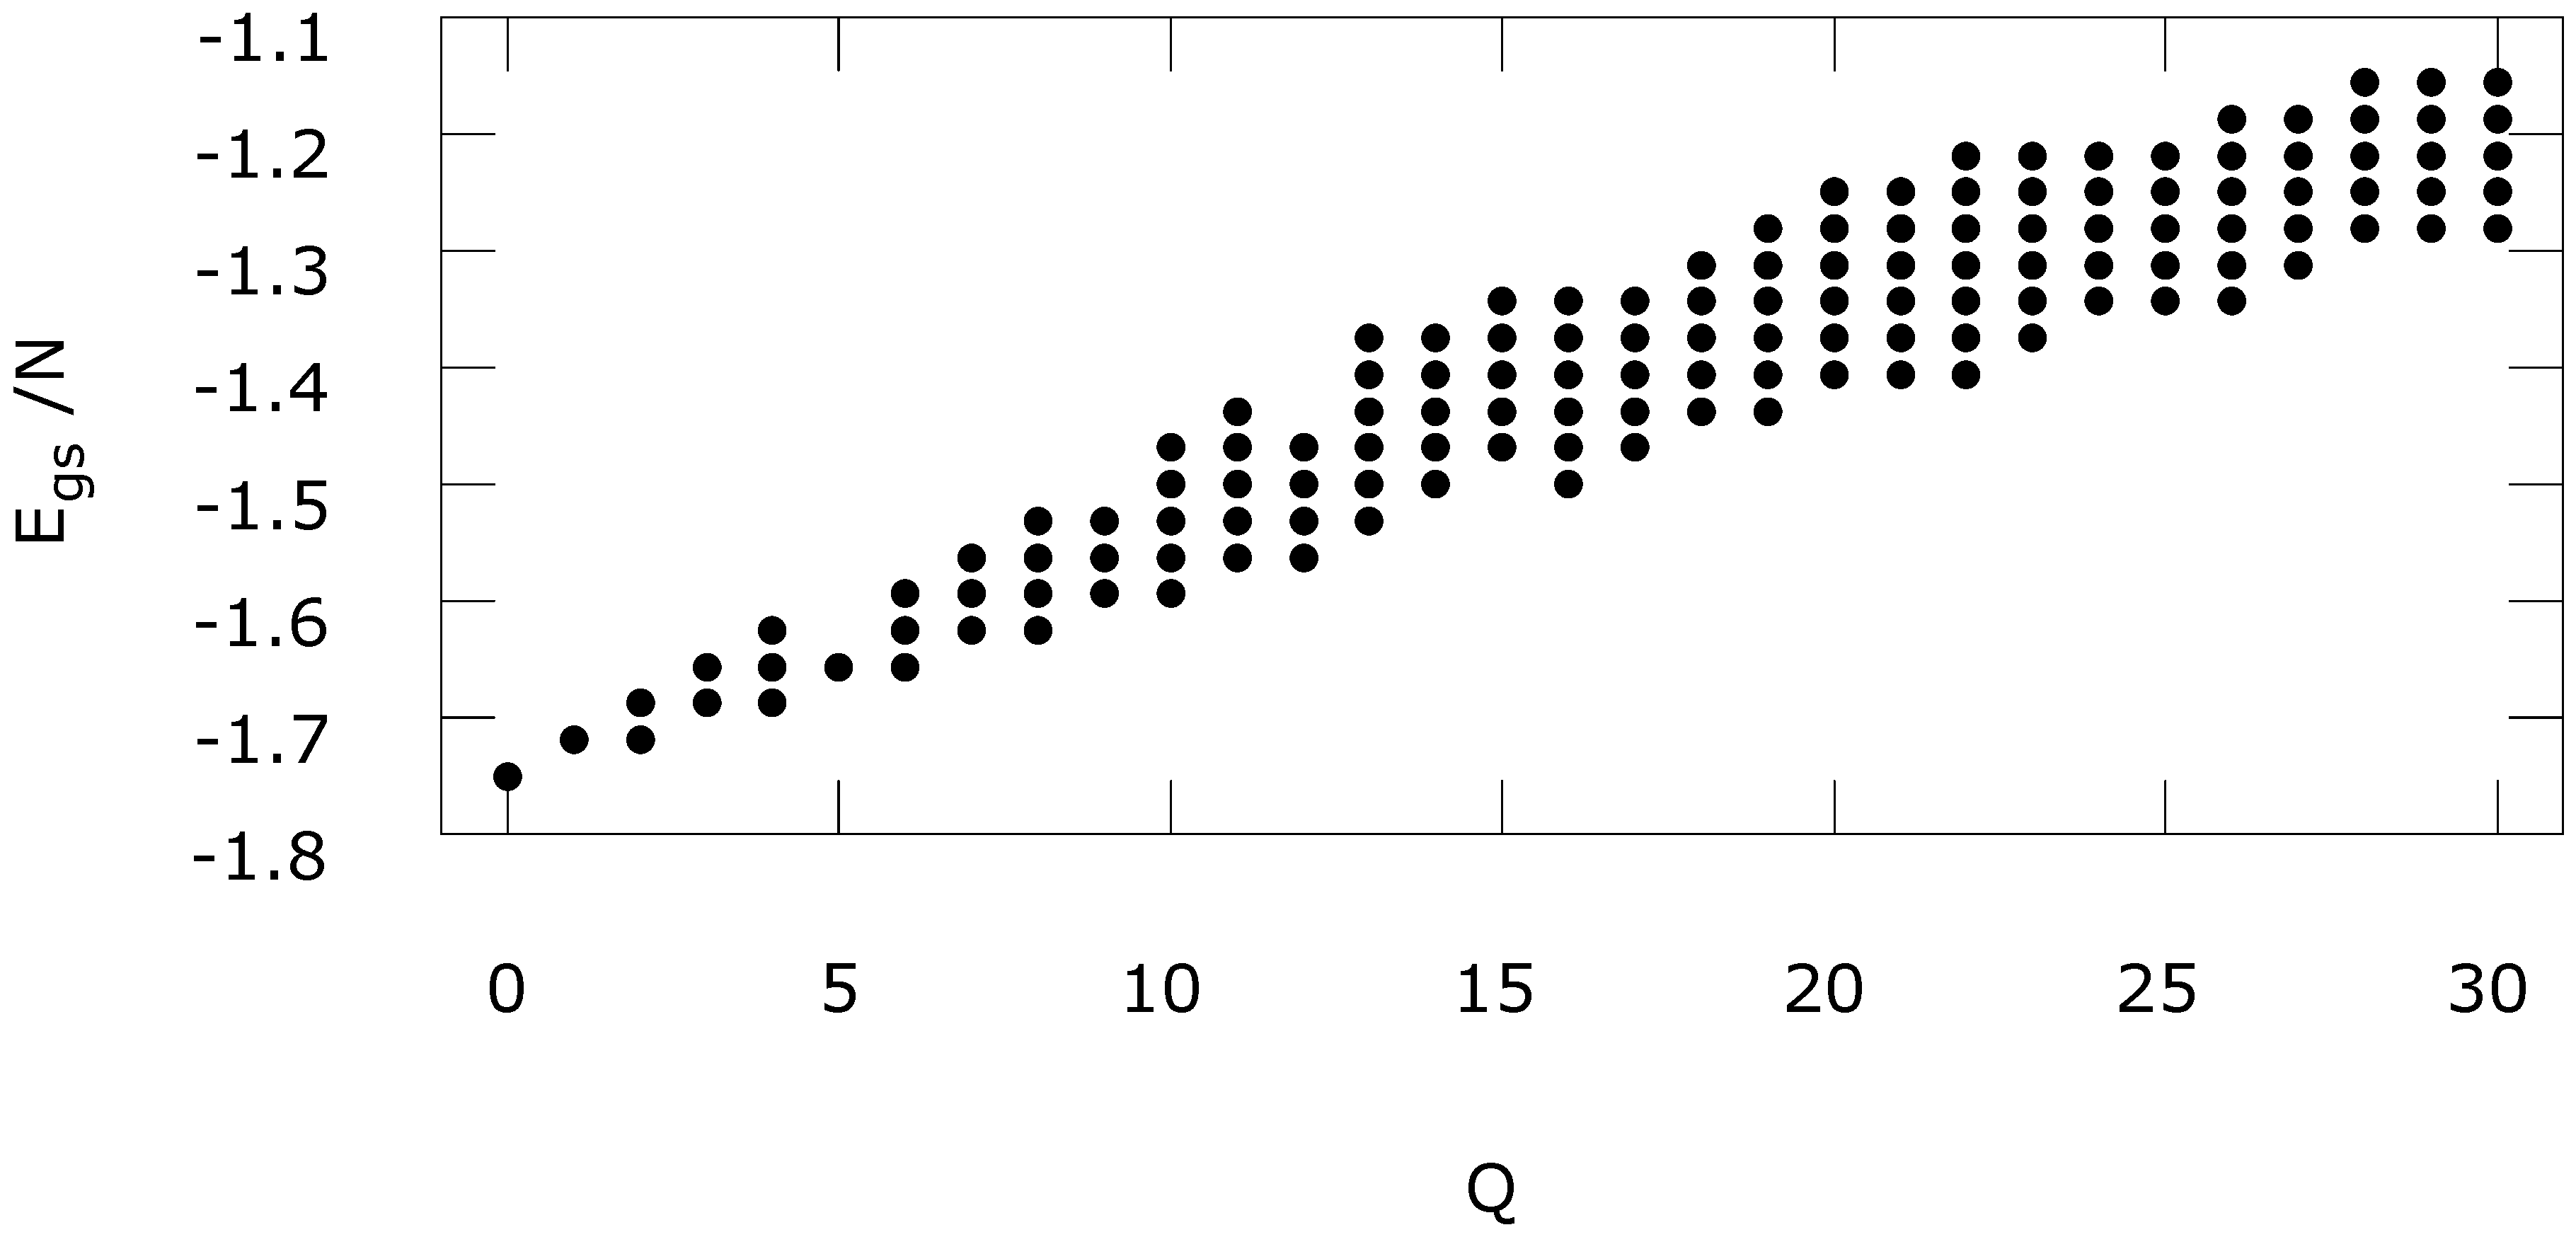
\includegraphics[width=0.9\linewidth]{pictures/E_Q.eps}
	\caption{Энергия основного состояния в зависимости от числа плакетов 2-го типа для $N=64$}
	\label{fig:E(Q)}
\end{figure}

С увеличением количества плакетов 2-го типа $Q$ энергия основного состояния увеличивается в среднем. На скорость увеличения энергии влияет не только количество плакетов 2-го типа, но и их расположение на решетке. Этим объясняется разброс значений энергий основного состояния на рисунке \ref{fig:E(Q)} и в таблице \ref{tab:Egs}.
Увеличение значения энергии основного состояния обусловлено ростом количества фрустраций с увеличением числа плакетов 2-го типа.

\begin{figure}[H]
	\centering
	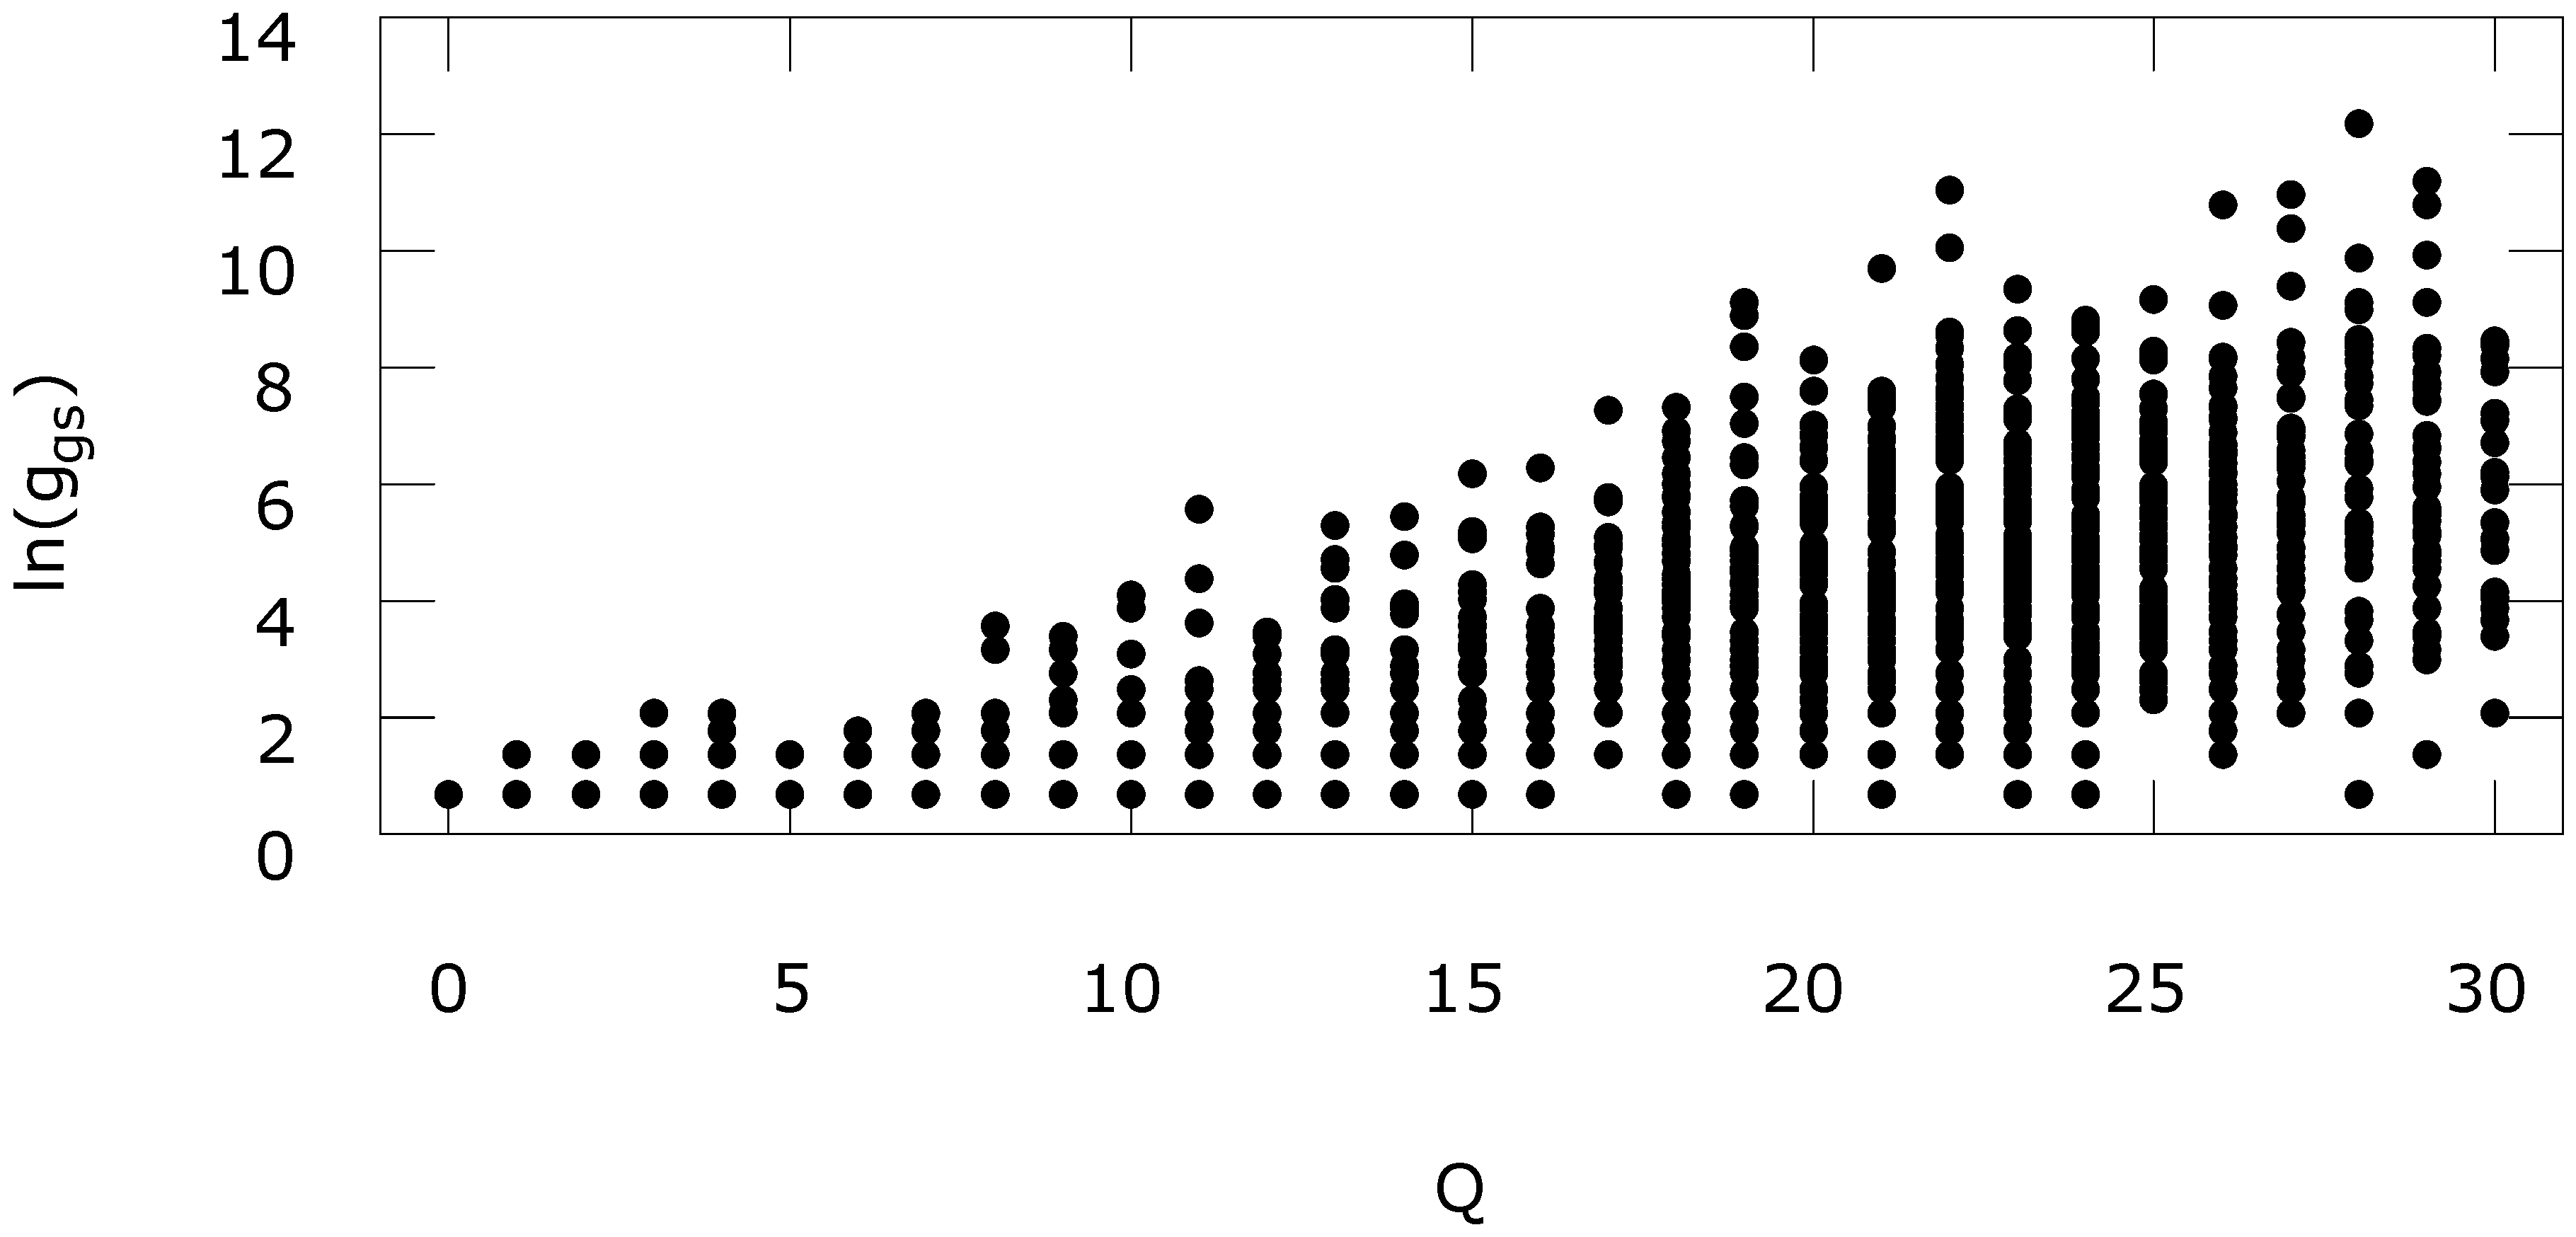
\includegraphics[width=0.9\linewidth]{pictures/g_Q.eps}
	\caption{Вырождение основного состояния в зависимости от числа плакетов 2-го типа для $N=64$}
	\label{fig:g(Q)}
\end{figure}

Увеличение числа плакетов 2-го типа и связанное с ним увеличение количества фрустраций в большинстве случаев ведет к увеличению вырождения основных состояний. Но для некоторых образцов увеличение количества фрустраций не вызывает рост вырождения основного состояния (см. точки с наименьшим значением $\ln{(g_{GS})}$ на рис. \ref{fig:g(Q)}). 

\section{Основное состояние во внешнем магнитном поле}

В таблице \ref{tab:Egs} приведены значения энергии основного состояния спинового стекла. Мы создали несколько образцов спинового льда, один из них на рисунке (\ref{fig:cell_SI_SG_64}) слева. Вычисления показывают, что энергия основного состояния на один спин при $P_+ = 0.5$ и отсутствии воздействия внешнего магнитного поля составила -0.97, при этом удельная энергия основного состояния спинового стекла в модели Эдвардса-Андерсона составила -1.28. Под спиновым льдом обычно понимается магнетики с периодичностью в обменных взаимодействиях \cite{peretyatko2017interplay, otsuka2018husimi, andriushchenko2019large, shevchenko2017effect, kato2022flux}. 

\begin{figure}[H]
	\begin{minipage}[h]{0.3\linewidth}
		\centering(a)
		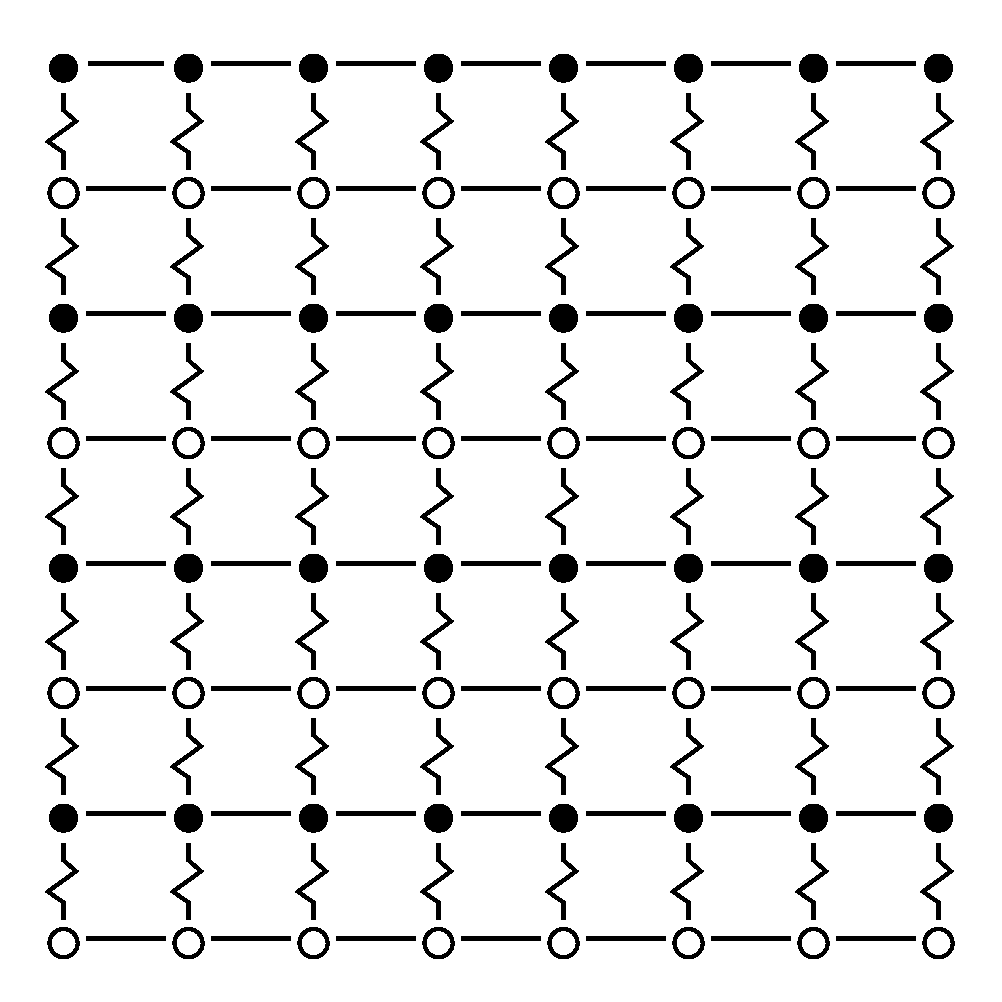
\includegraphics[width=1\linewidth]{pictures/SI_64_J0_1}
	\end{minipage}
	\hfill
	\begin{minipage}[h]{0.3\linewidth}
	\centering(b)
	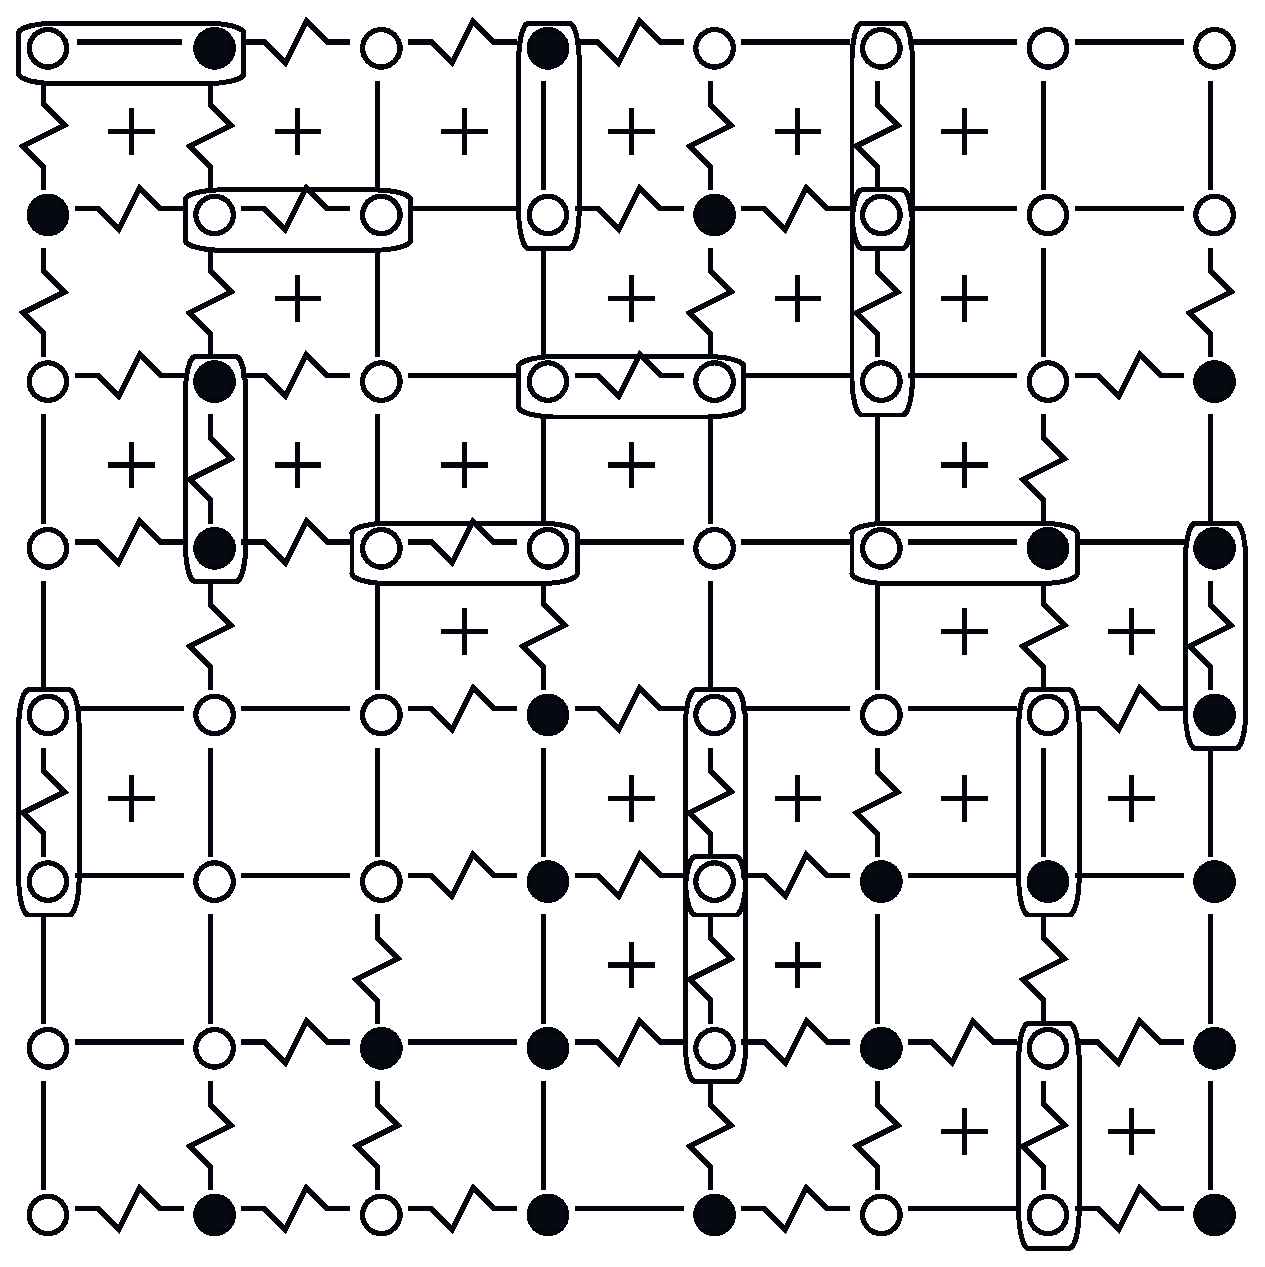
\includegraphics[width=1\linewidth]{pictures/SG_64_J0}
	\end{minipage}
	\hfill
	\begin{minipage}[h]{0.3\linewidth}
		\centering(c)
		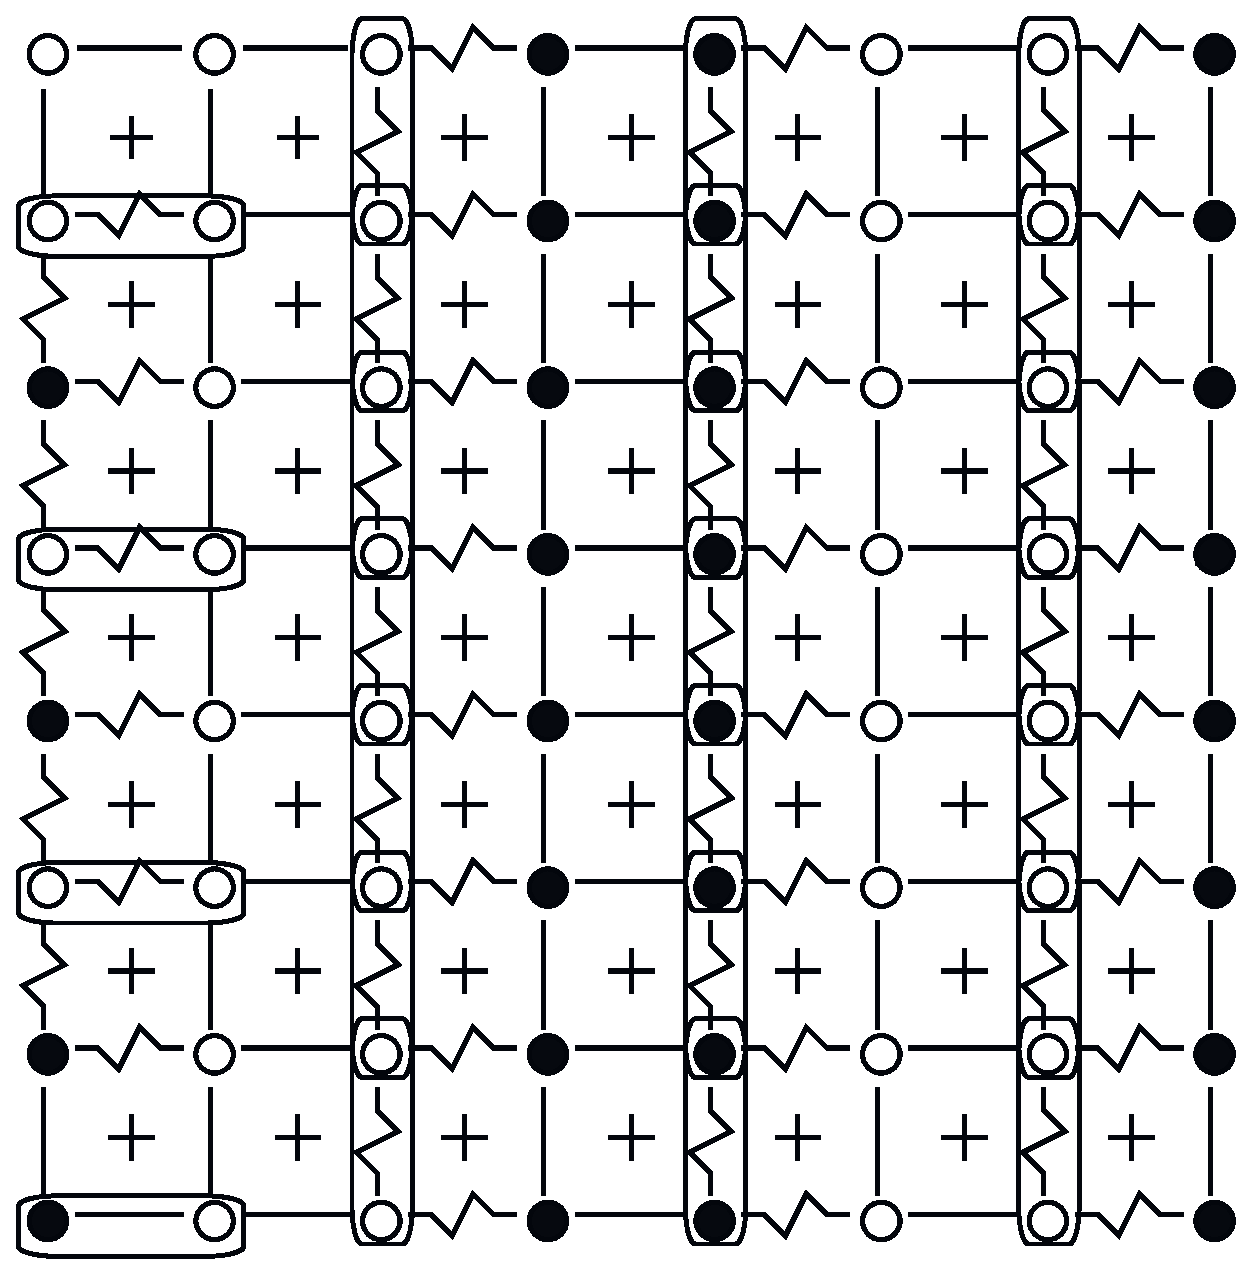
\includegraphics[width=1\linewidth]{pictures/SI_64_J0}
	\end{minipage}
	\hfill
	\caption{Спиновый лед (a,c) и спиновое стекло (b), 64 спина, $P_+ = 0.5$}
	\label{fig:cell_SI_SG_64}

\end{figure}


На рисунке \ref{fig:cell_SI_SG_64}(a) представлена плоская решетка спинового льда, составленная из плакетов 1-го типа, в которой полностью отсутствуют фрустрации. 

На рисунке \ref{fig:cell_SI_SG_64}(b) представлена решетка спинового стекла, в которой из 49 плакетов имеется 16 плакетов 1-го типа, 27 - 2-го типа и 6 плакетов 3-го типа. Всего 15 фрустраций.

В решетке спинового льда на рисунке \ref{fig:cell_SI_SG_64}(c) максимальное количество фрустраций, в данном примере, достигается путем заполнения системы плакетами 2-го типа. Всего 25 фрустраций на 49 плакетов.


\begin{figure}[H]
	\begin{minipage}[h]{0.32\linewidth}
		\centering(a)
		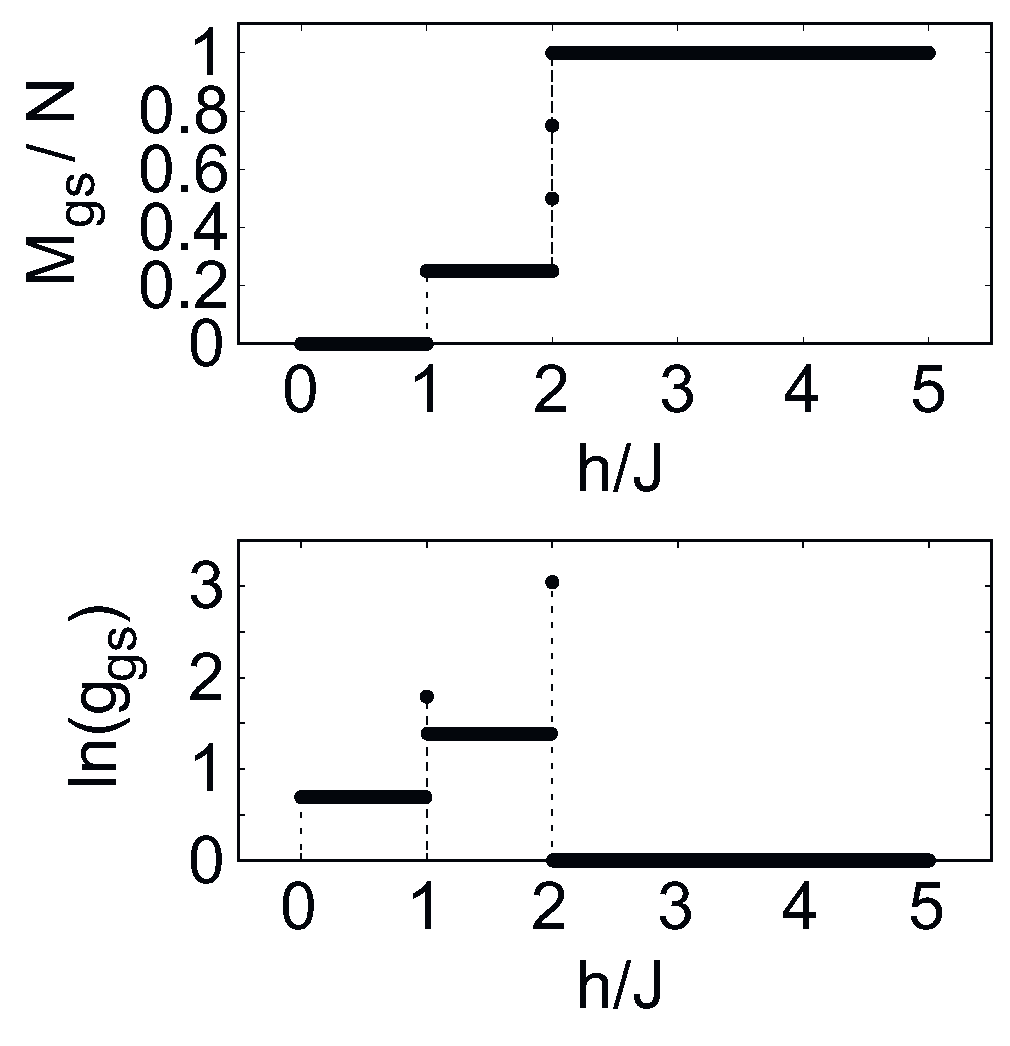
\includegraphics[width=1\linewidth]{pictures/_multiplot_SI64_J0_1}
	\end{minipage}
	\hfill
	\begin{minipage}[h]{0.32\linewidth}
		\centering(b)
		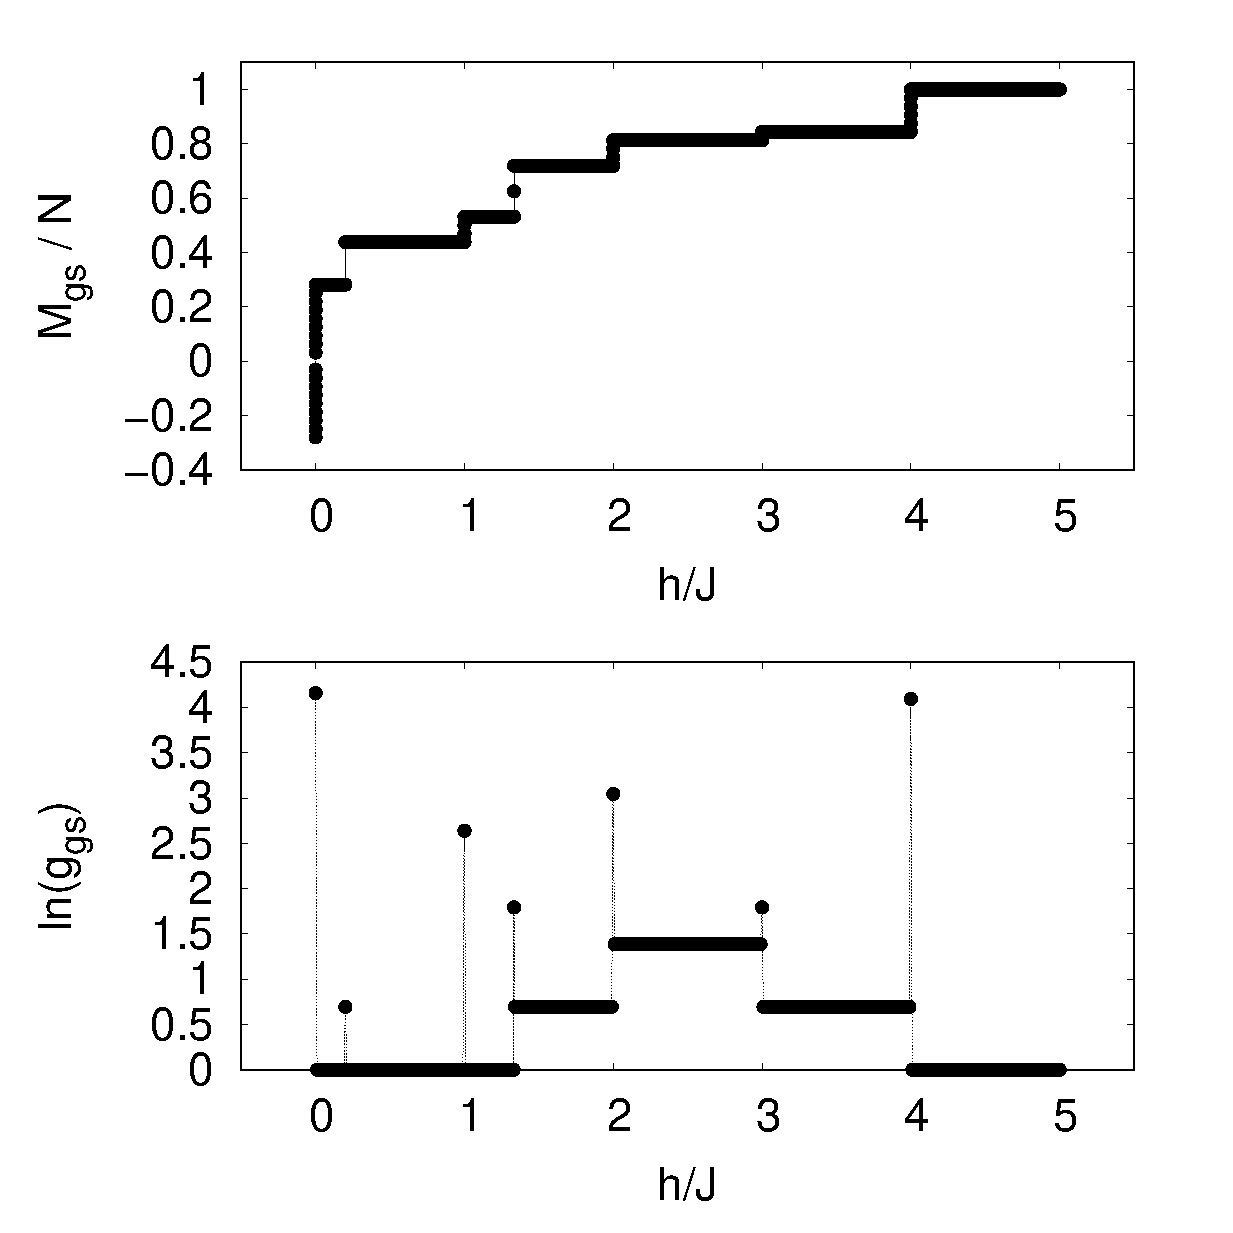
\includegraphics[width=1\linewidth]{pictures/_multiplot_SG64_J0}
	\end{minipage}
	\hfill
	\begin{minipage}[h]{0.32\linewidth}
		\centering(c)
		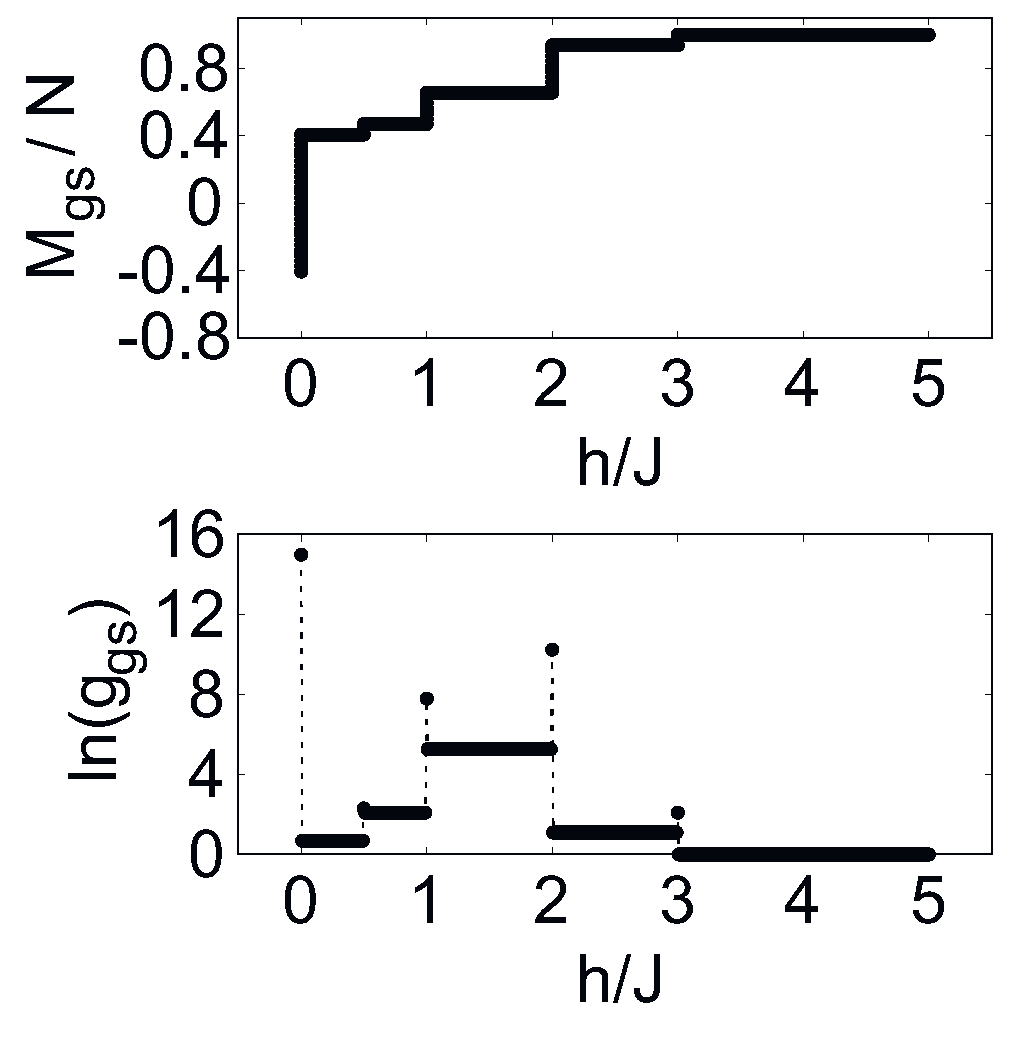
\includegraphics[width=1\linewidth]{pictures/_multiplot_SI64_J0}
	\end{minipage}
	
	\caption{Спиновый лед (a, c) и спиновое стекло (b), 64 спина, $P_+ = 0.5$}
	\label{fig:_multiplot_SI_SG_64}
	
\end{figure}


На рисунке \ref{fig:_multiplot_SI_SG_64} представлены зависимости спинового избытка и вырождение основного состояния от значения напряженности внешнего магнитного поля. 

При отсутствии фрустраций и внешнего магнитного поля основное состояние спинового льда вырождено дважды (рисунок \ref{fig:_multiplot_SI_SG_64}(a)).

В системе спинового стекла с появлением фрустраций вырождение основного состояния достигает 64 состояний (рисунок \ref{fig:_multiplot_SI_SG_64}(b)).

Максимальное заполнение системы спинового льда фрустрированными плакетами 2-го типа приводит к макроскопическому вырождению основного состояния, количество вырождений достигает 3211264 конфигураций (рисунок \ref{fig:_multiplot_SI_SG_64}(c)).



При воздействии внешнего магнитного поля больше всего ступенек на графике спинового избытка наблюдается в системе спинового стекла (рисунок \ref{fig:_multiplot_SI_SG_64}(b)). Причем их количество обуславливается не множеством фрустраций, а формой плотности распределения состояний (DOS), которая играет важную роль.
Стоит заметить, что количество ступенек не явным образом зависит от числа фрустраций.


Методом исчерпывающего перечисления для образцов спинового льда и спинового стекла, представленных на рис. \ref{fig:cell_SI_SG_64}, были построены плотности распределения состояний в зависимости от значений внешнего магнитного поля (рис. \ref{fig:HDOS_ice_1}, \ref{fig:HDOS_glass} и \ref{fig:HDOS_ice}).
Энергия системы с учетом воздействия внешнего магнитного поля вычислялась по формуле (\ref{eq:ising_energy}).




\begin{figure}[H]
	\centering
	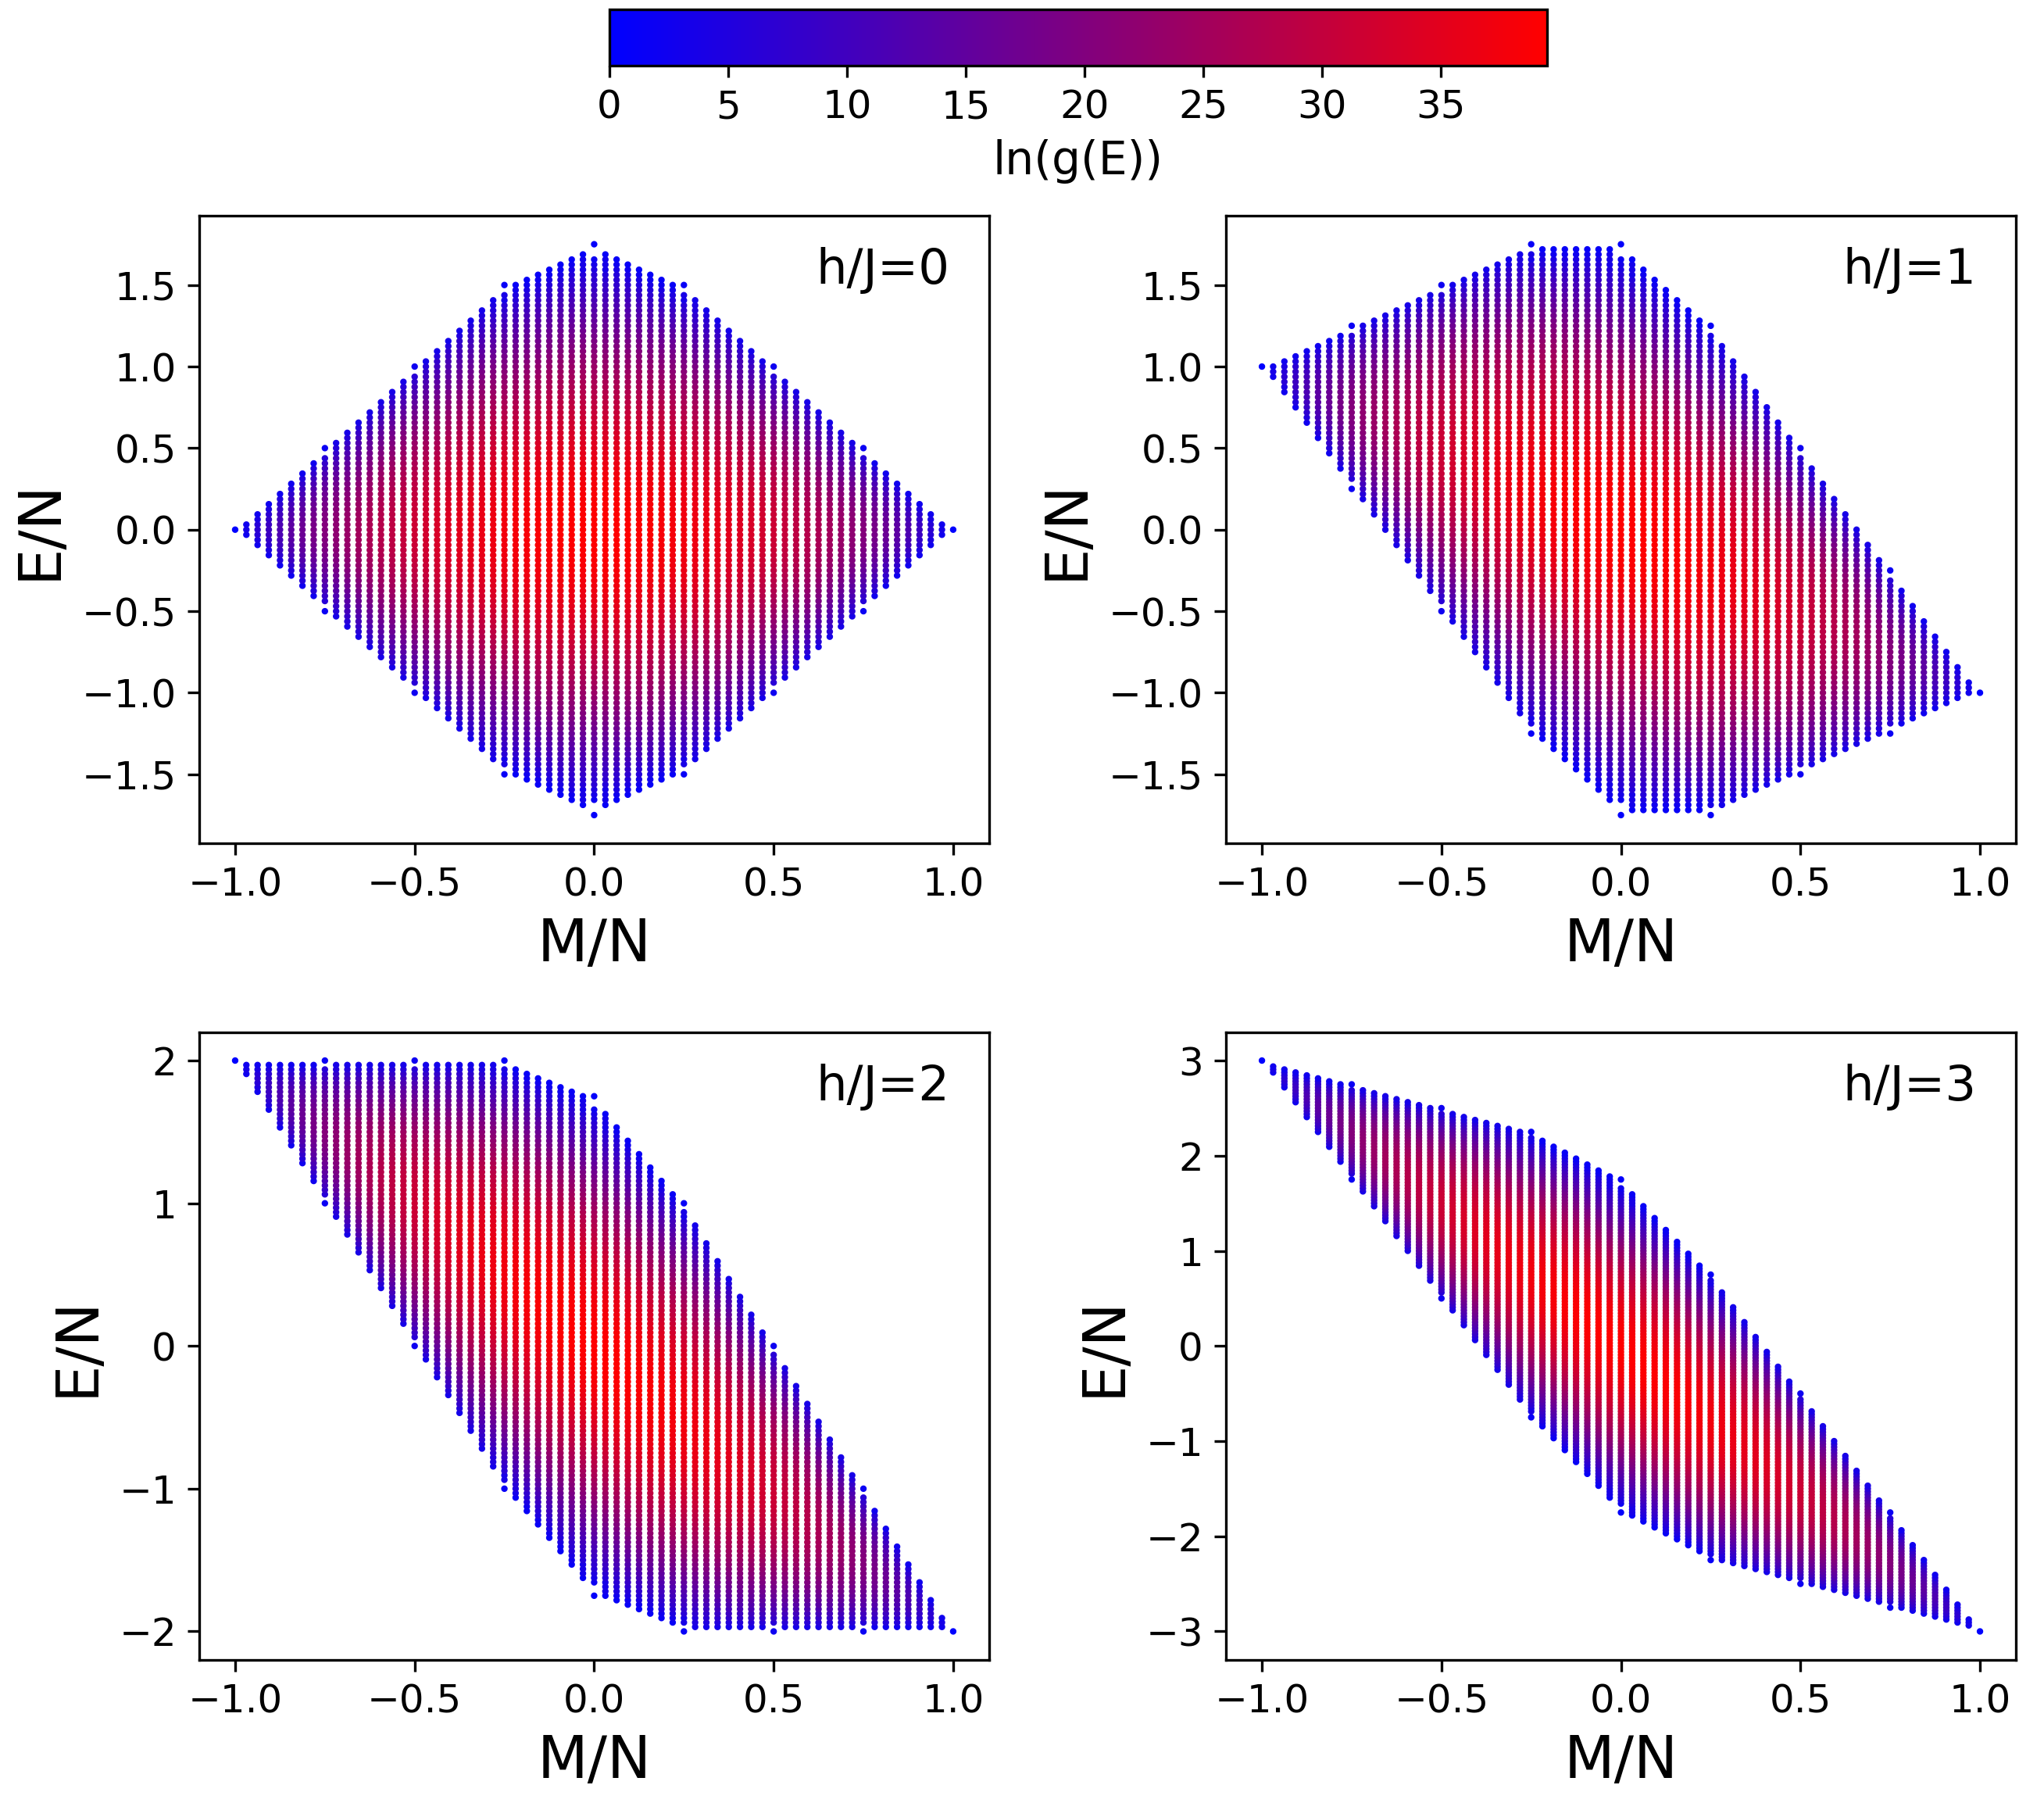
\includegraphics[width=1\linewidth]{pictures/HDOS_SI_64_J0_1.png}
	\caption{DOS, h/J=0-2, Спиновый лед, 64 спина, $P_+ = 0.5$}
	\label{fig:HDOS_ice_1}
\end{figure}




\begin{figure}[H]
		\centering
		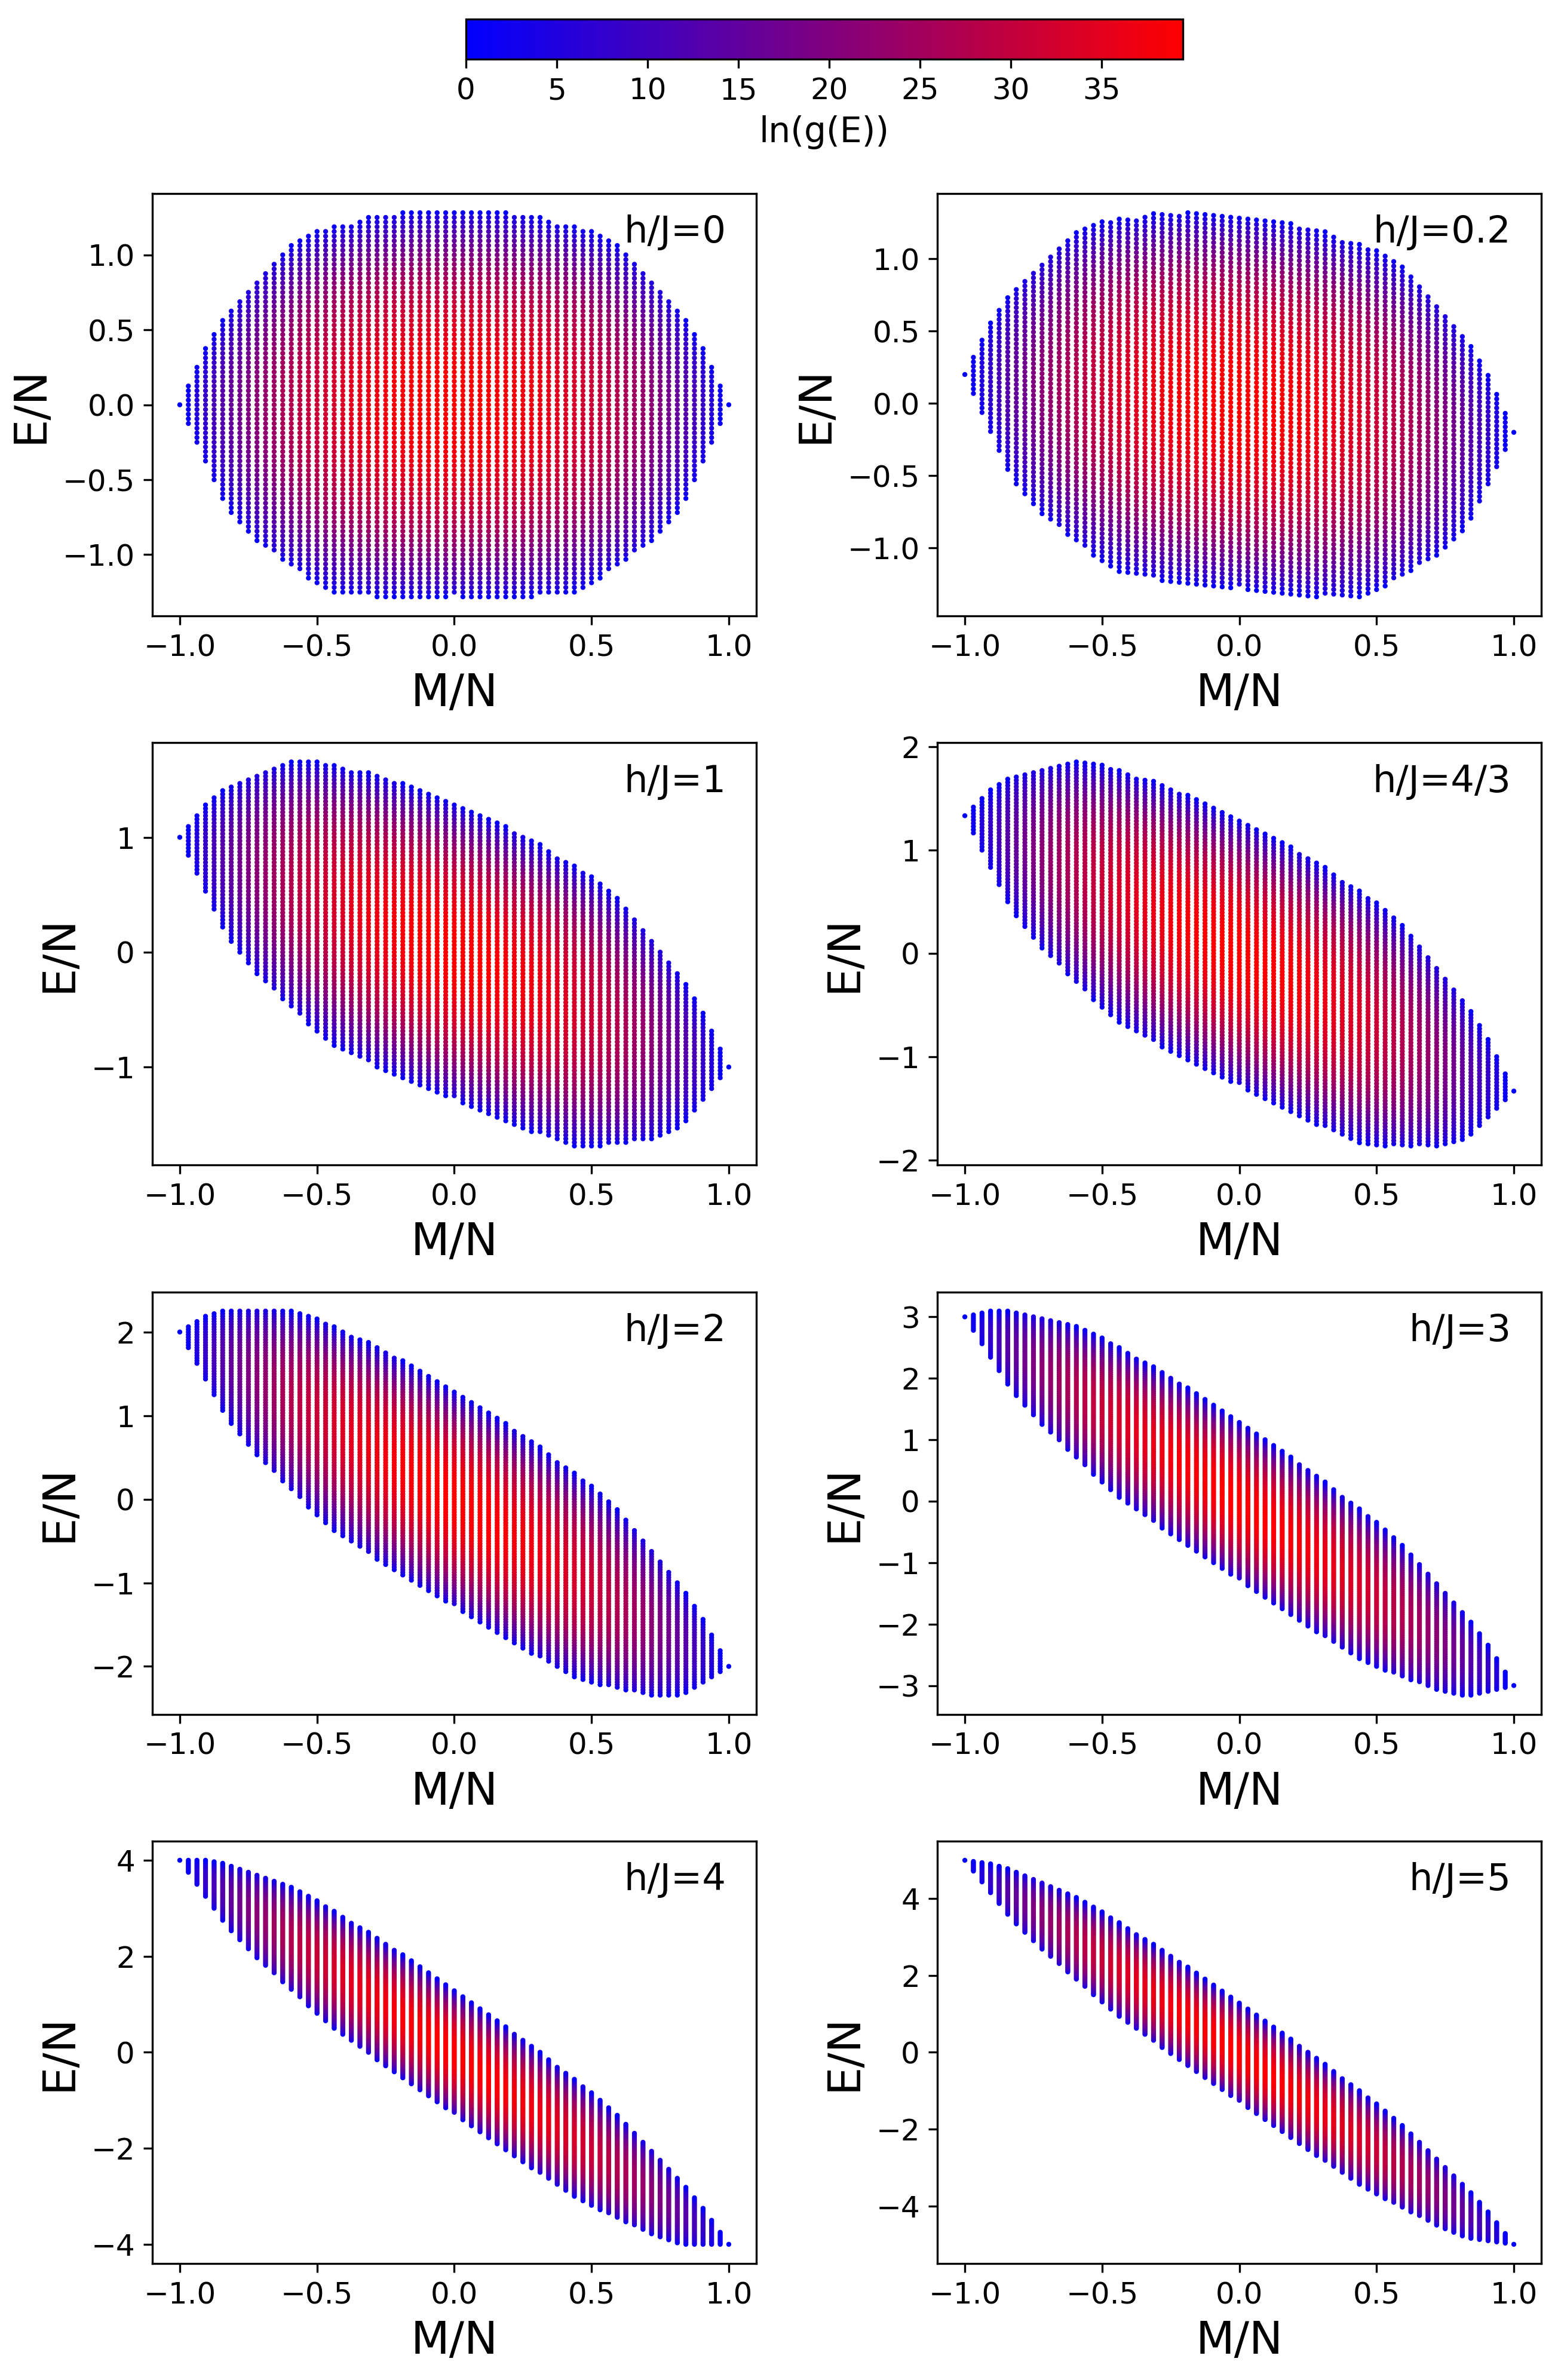
\includegraphics[width=1\linewidth]{pictures/HDOS_SG_64_J0.png}
	\caption{DOS, h/J=0-5, Спиновое стекло, 64 спина, $P_+ = 0.5$}
	\label{fig:HDOS_glass}
\end{figure}


\begin{figure}[H]
	\centering
	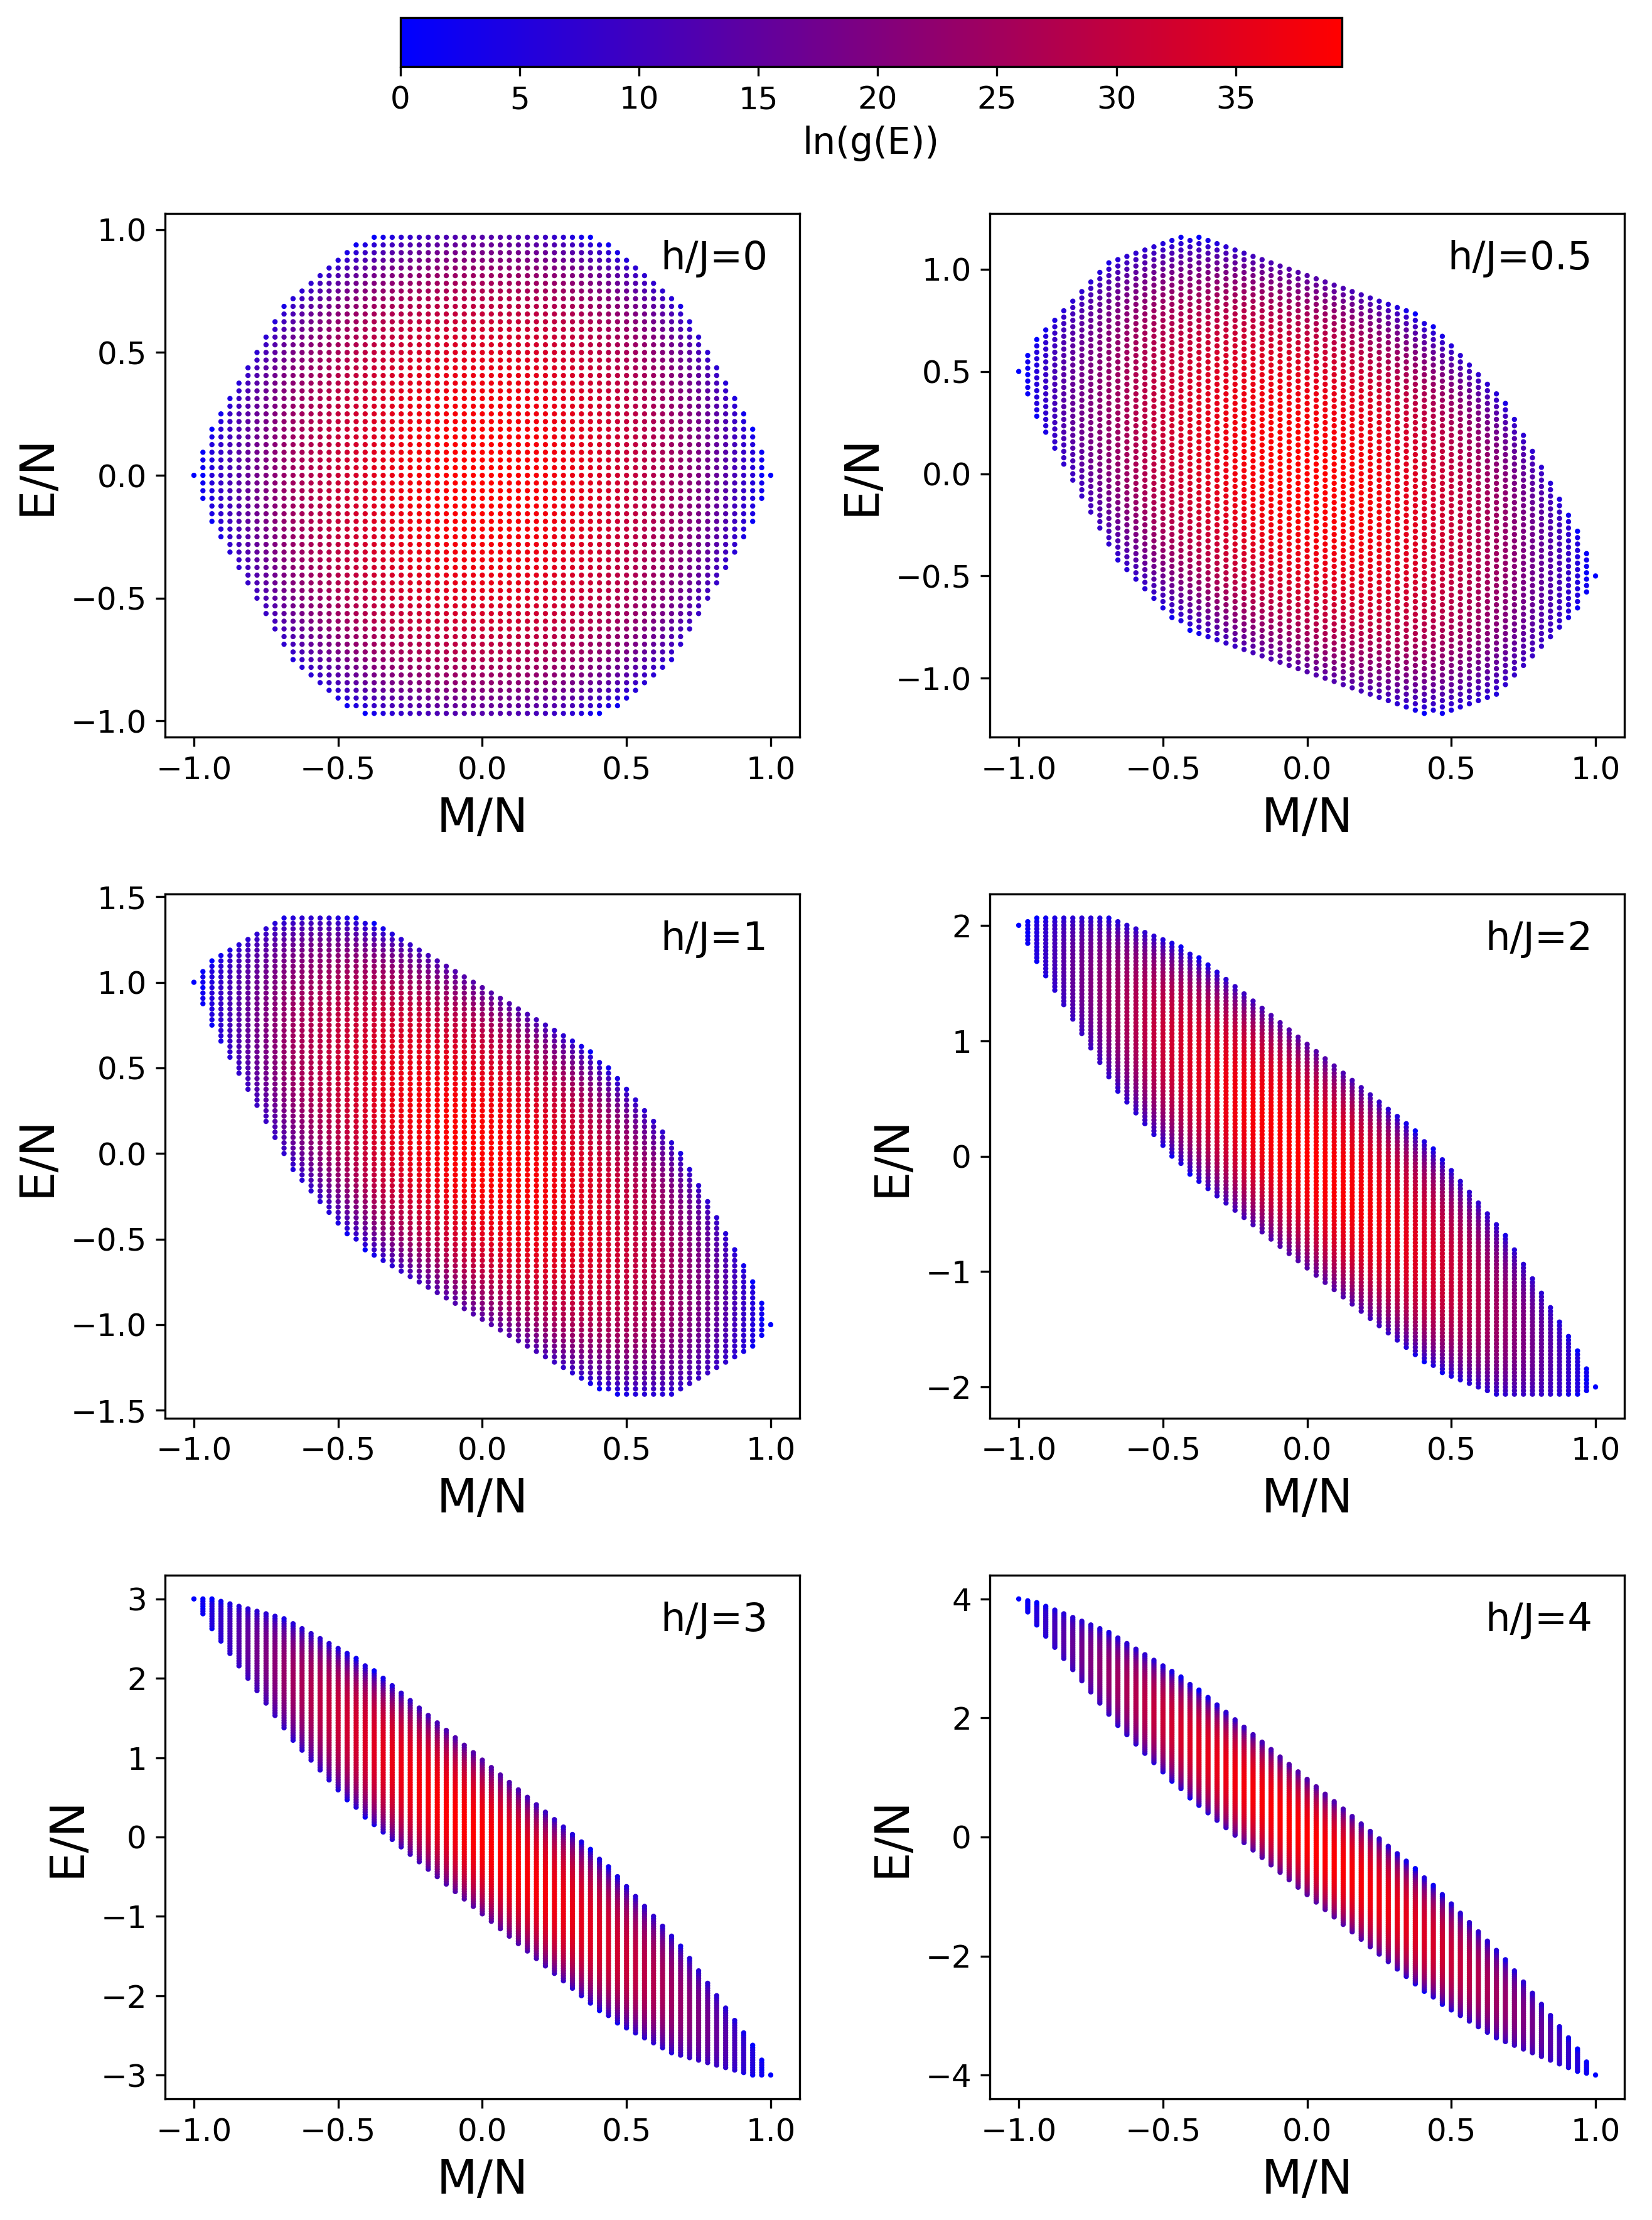
\includegraphics[width=1\linewidth]{pictures/HDOS_SI_64_J0.png}
	\caption{DOS, h/J=0-4, Спиновый лед, 64 спина, $P_+ = 0.5$}
	\label{fig:HDOS_ice}
\end{figure}


Как мы можем видеть на рисунке \ref{fig:cell_SI_SG_64} при $h/j=0$ для спинового льда (рис. \ref{fig:_multiplot_SI_SG_64}(a)) можно видеть вырождение основного состояния. Увеличение до значения внешнего магнитного поля до критического значения $h/j=1$ за счет увеличения энергии Зеемана приводит к тому, что энергия основного состояния со спиновым избытком $M=0$ сравнивается с энергией основного состояния со спиновым избытком $M=0.25$. Энтропии основных состояний складываются.

Увеличение значения внешнего магнитного поля до $h/j=2$ приводит к ситуации, когда основными состояниями становятся состояния со спиновыми избытками $M=\pm0.25; \pm0.5; \pm0.75; \pm1$.

Значение  $h/j=3$ есть поле насыщения, при котором остается только одна конфигурация.


Для спинового стекла (рис. \ref{fig:cell_SI_SG_64}(b)) скачки энтропии при $T=0$ в критических полях $h/j=0.2; 1; 4/3; 2; 3; 4; 5$ обусловлены границами плотности состояний (см. рис. \ref{fig:HDOS_glass}, $h/j=0$).


Спиновый лед (рис. \ref{fig:cell_SI_SG_64}(c)) имеет не такое большое разнообразие критических полей в отличие от спинового стекла (см. рис. \ref{fig:HDOS_glass}). Однако вырождение основных состояний намного более высокое.

\todo{???Вопросы размещения фрустраций в конфигурациях основного состояния, их подавления внешним магнитным полем для конфигураций основного состояния в поле.
(посмотреть вырождение)}


\section{Состояния при $T = 0$}

В работе \cite{trukhin4855337thermodynamic} определена фазовая диаграмма при отличной от нуля температуре во внешнем магнитном поле. Представляет интерес вопрос разделения фаз спинового стекла, ферромагнетика и антиферромагнетика при $T=0$.

В таблице \ref{tab:lit_phase} представлены данные теоретических и численных расчётов критической точки перехода (относительная концентрация ферромагнитных связей $P_+$) из фазы антиферромагнетика в фазу спинового стекла.

\begin{table}[!h]
	\begin{tabular}{|l|c|l|}
		\hline
		Method                                   & $P_{+}$                                       & Reference                                           
		\\ \hline
		Series expansion 								& ~0.099                                  & \cite{PhysRevB.19.260}    \\ \hline
	     Matching algorithm                            & 
	     0.105 $\pm 0.01$                                        & \cite{H_Freund_1989} \\ \hline
		Matching algorithm                      & 
		$0.095<p_c<0.108$                                          & \cite{BENDISCH1994139}      \\ \hline
		Exact ground states                       & 
		$0.106 \pm 0.002$                               & \cite{N.Kawashima_1997}     \\ \hline
		Ground state enumeration                             & 0.115                                          & \cite{PhysRevE.58.1502} \\ \hline
    	Exact ground states        & 
		$0.1031\pm0.0001$                                          & \cite{WANG200331}   \\ \hline
		Exact ground states   & $0.103\pm0.001$                                       & \cite{amoruso2004domain} 
		    \\ \hline
			
	\end{tabular}
	\caption{Критическая концентрация ферромагнитных связей}
	\label{tab:lit_phase}
\end{table}

На рисунке \ref{fig:Mgs(P+)} представлена диаграмма спиновых избытков основного состояния образцов квадратной решетки Изинга, которая получена на основе данных исчерпывающего перечисления. Плотность распределения ферромагнитных связей определяется параметром $P_+$. Связи распределены случайным образом с сохранением $P_+$ для одной серии. Каждая серия содержала \textbf{10 образцов} для численного расчёта. 

\begin{figure}[H]
	\centering
	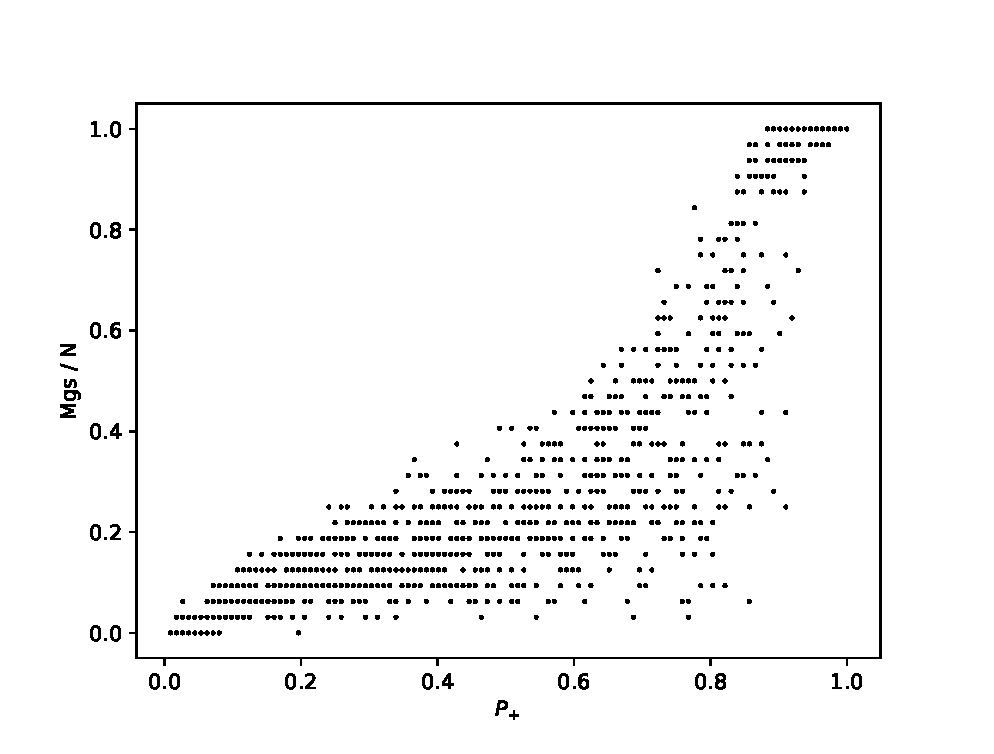
\includegraphics[width=0.8\textwidth]{images/Mgs(P+).eps}
	\caption{Значения максимального спинового избытка основного состояния в зависимости от относительного количества ферромагнитных связей}
	\label{fig:Mgs(P+)}
\end{figure}

Очевидно, что для чистого ферромагнетика спиновый избыток будет равен количеству спинов, а для чистого антиферромагнетика нулю (в случае чётного количества спинов). Для каждого заданного $P_+$ отношение числа точек, в которых максимальный спиновый избыток основного состояния равен нулю к числу точек, где $M_{gs}/N \neq 0.0$ есть вероятность антиферромагнитного состояния (рис. \ref{fig:P_AFM_FM_Mmax} a). Аналогичным образом отношение числа точек с $M_{gs}/N = 1.0$ ферромагнитных спиновых избытков основного состояния к числу точек когда $M_{gs}/N \neq 1.0$ есть вероятность ферромагнитного состояния (рис. \ref{fig:P_AFM_FM_Mmax} b).

\begin{figure}[H]
	\begin{minipage}[h]{0.45\linewidth}
		\centering $(a)$
		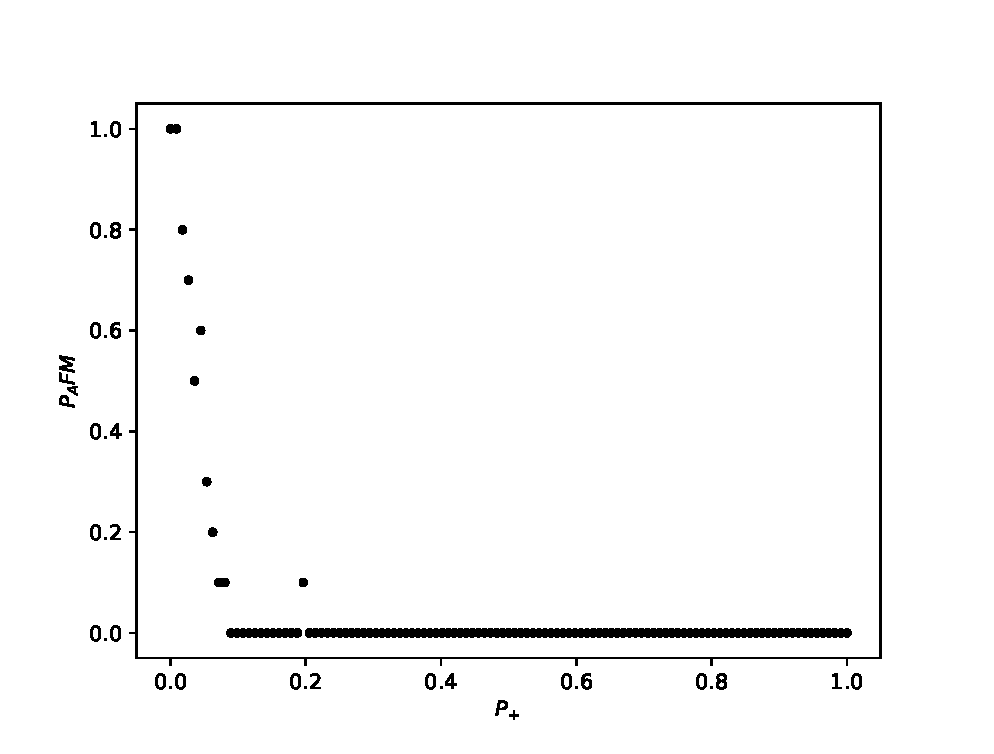
\includegraphics[width=1\linewidth]{images/P_AFM_Mmax.eps}
	\end{minipage}
	\hfill
	\begin{minipage}[h]{0.45\linewidth}
		\centering $(b)$
		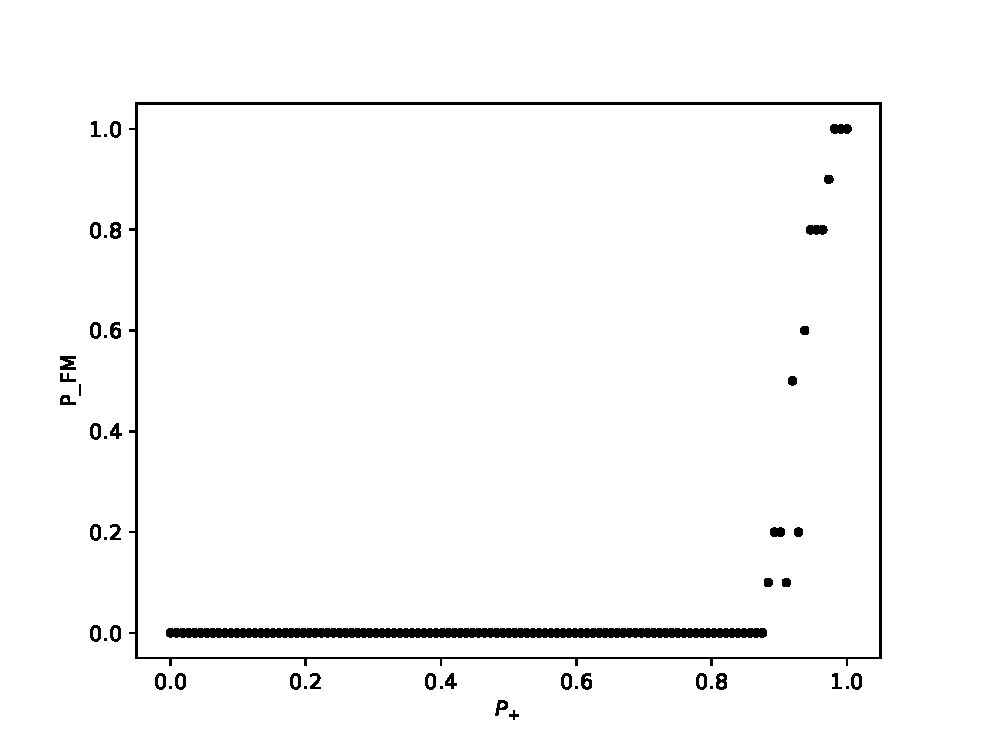
\includegraphics[width=1\linewidth]{images/P_FM_Mmax.eps}
	\end{minipage}
	\caption{Вероятность антиферромагнитного (a) и ферромагнитного (b) состояния}
	\label{fig:P_AFM_FM_Mmax}
\end{figure}

Антиферромагнитная фаза при $T = 0$ реализуется при $0.0 \leq P_+ \leq 0.1$. Спиновое стекло реализуется при $0.1 \leq P_+ \leq 0.9$. Ферромагнитная фаза, реализуется при $0.9 \leq P_+ \leq 1.0$. Полученные значения отделяют антиферромагнитную фазу в тех же значениях $P_+$ что и в работах представленных в таблице \ref{tab:lit_phase}, а так же позволяют отделить ферромагнитную фазу в нулевой температуре.

todo: попробовать пересчитать из вырождений, а не линий M
\begin{comment}
Другим возможным подходом к разделению фаз может служить вырождение основного состояния (рис. \ref{fig:Ggs}). Известно, что основные состояния антиферромагнетика имеют одни занчения M, а ферромагнетика вырождено ровно в два варианта. Можем найти вероятности быть антиферромагнетиком или ферромагнетиком посчитав отношения вырождения $G_{gs} = 1$ ко всем и $G_{gs} = 2$ ко всем, соответственно. Полученные диаграммы представлены на рисунке \ref{fig:P_AFM_FM_G(Mgs)}

\begin{figure}[H]
	\centering
	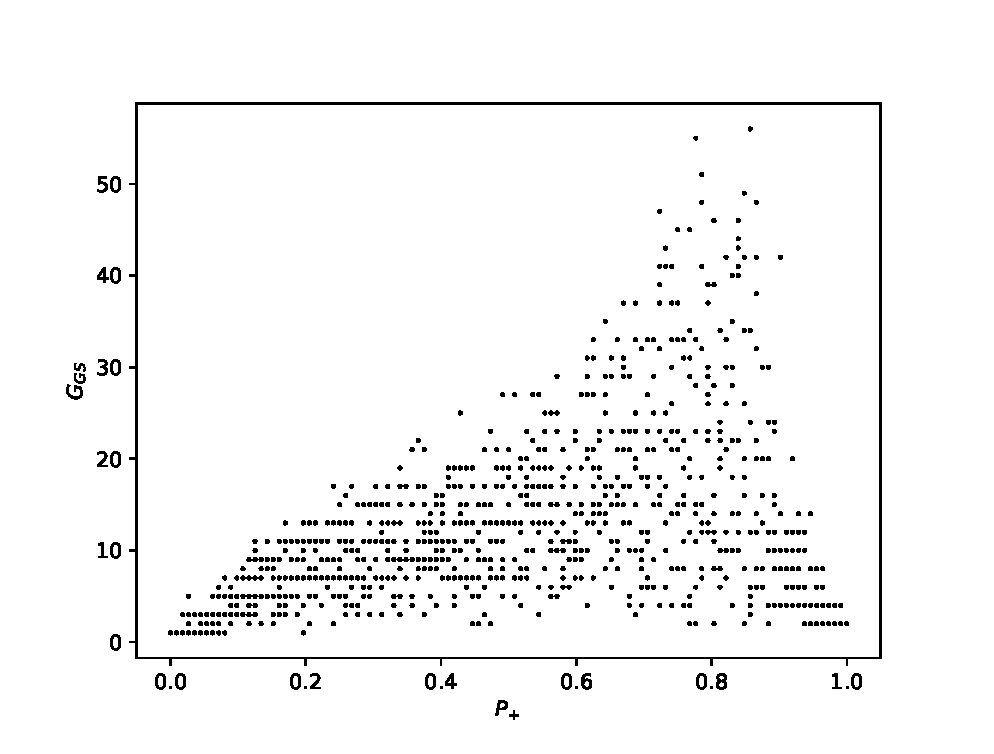
\includegraphics[width=0.8\textwidth]{images/Ggs.eps}
	\caption{}
	\label{fig:Ggs}
\end{figure}



\begin{figure}[H]
	\begin{minipage}[h]{0.45\linewidth}
		\centering $(a)$
		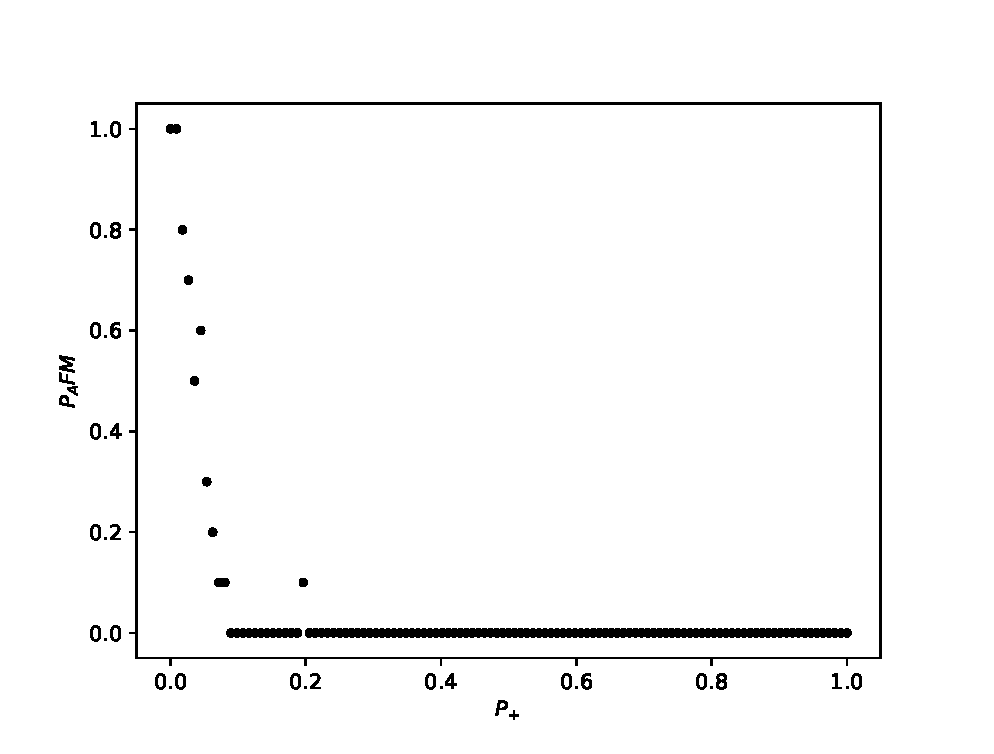
\includegraphics[width=1\linewidth]{images/P_AFM_G(Mgs).eps}
	\end{minipage}
	\hfill
	\begin{minipage}[h]{0.45\linewidth}
		\centering $(b)$
		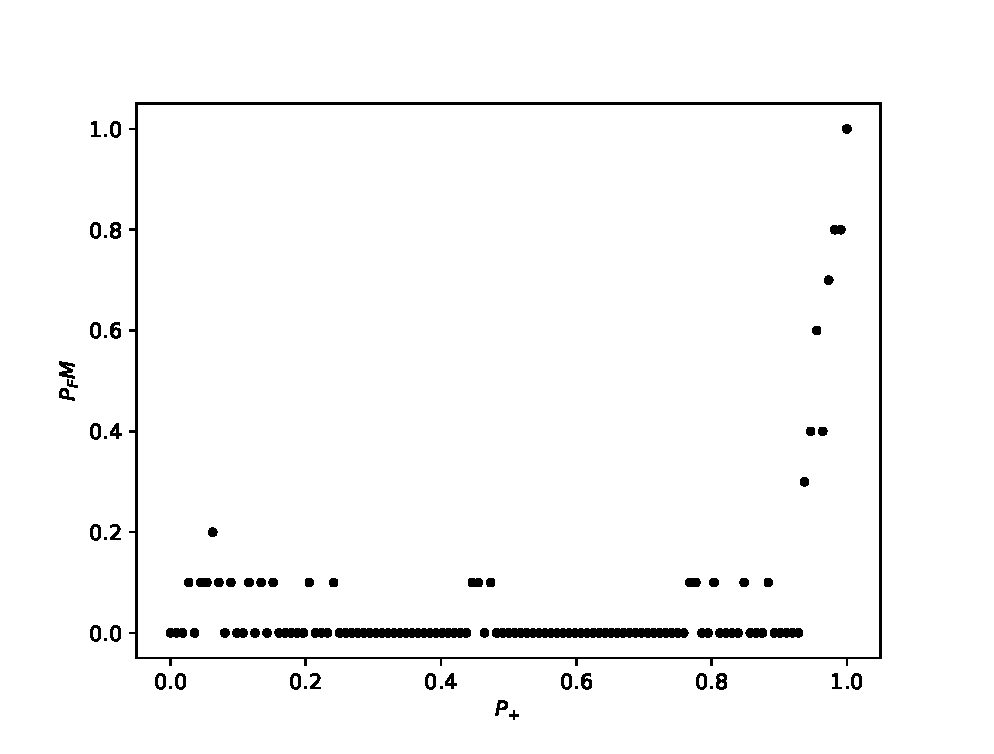
\includegraphics[width=1\linewidth]{images/P_FM_G(Mgs).eps}
	\end{minipage}
	\caption{Вероятность антиферромагнитного (a) и ферромагнитного (b) состояния}
	\label{fig:P_AFM_FM_G(Mgs)}
\end{figure}
\end{comment}

Полная плотность состояний позволяет достоверно рассчитать свойства образцов во внешнем магнитном поле. Так диаграмма спиновых избытков основного состояния образцов плоской решетки Изинга \ref{fig:Mgs(P+)} в внешнем магнитом поле $H = 1$ и $H = 2$ в единицах $J$ представлен на рисунке \ref{fig:Mgs(P+)_H}.

todo: переделать в график P+(h)
\begin{figure}[H]
	\begin{minipage}[h]{0.45\linewidth}
		\centering $(a)$
		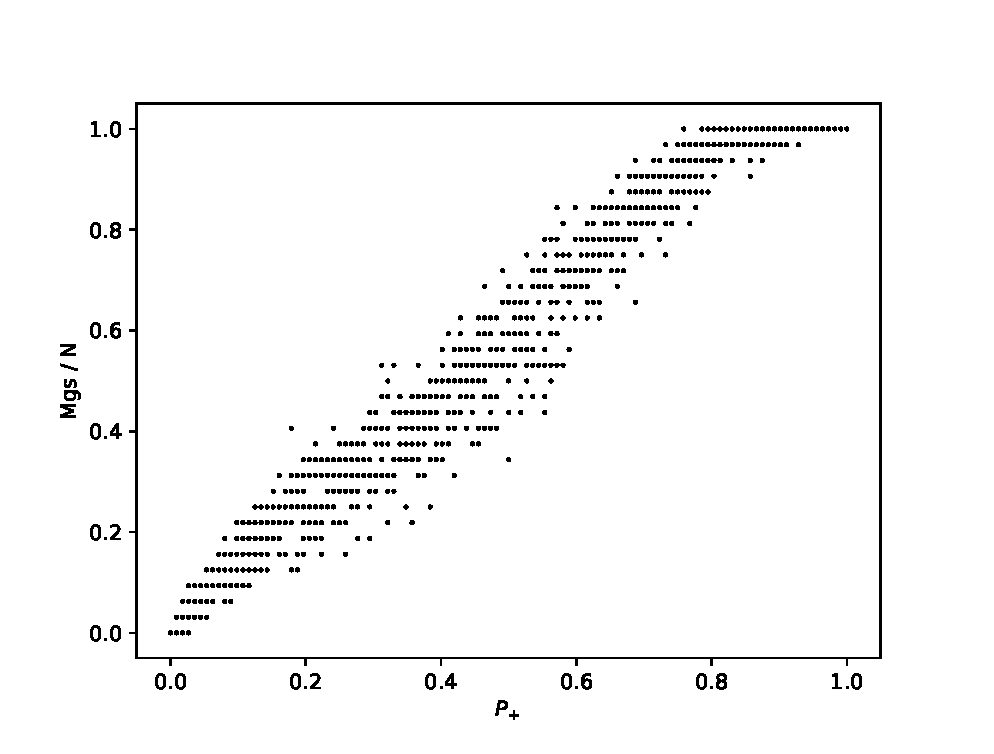
\includegraphics[width=1\linewidth]{images/Mgs(P+)_H1.eps}
	\end{minipage}
	\hfill
	\begin{minipage}[h]{0.45\linewidth}
		\centering $(b)$
		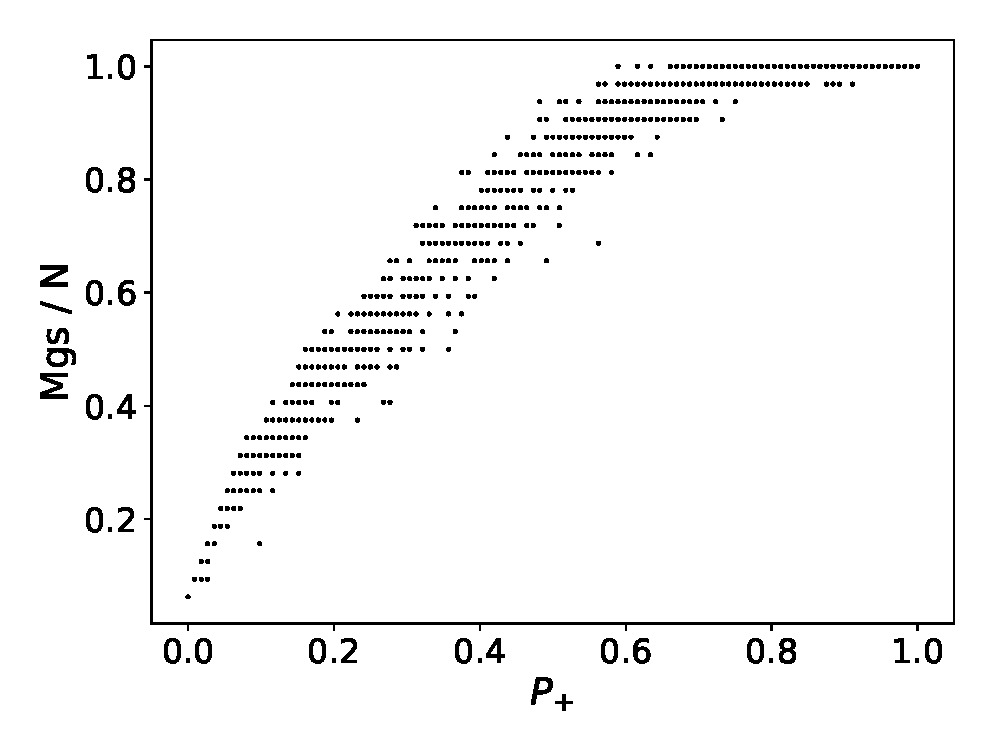
\includegraphics[width=1\linewidth]{images/Mgs(P+)_H2.eps}
	\end{minipage}
	\caption{Спиновый избыток основного состояния для всех значений плотности распределения обменных интегралов во внешнем магнитном поле $H = 1$ (a) и $H = 2$ (b)}
	\label{fig:Mgs(P+)_H}
\end{figure}

Вариант графика P+(h) (рис. \ref{fig:P+_afm_fm(H)}):

\begin{figure}[H]
	\centering
	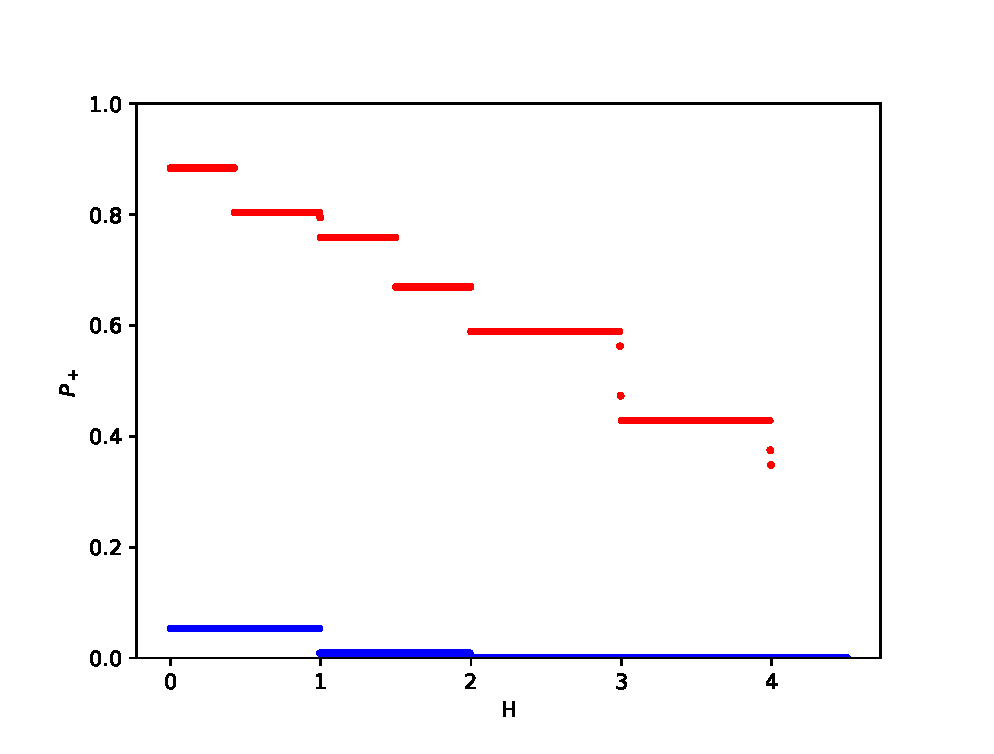
\includegraphics[width=0.8\textwidth]{images/P+_afm_fm(H).eps}
	\caption{Красная линия -- фазовый переход в ферромагнетик. Синяя -- в антиферромагнетик}
	\label{fig:P+_afm_fm(H)}
\end{figure}

\section{Заключение}

С помощью разработанных программ ЭВМ на основании авторского подхода, а также с помощью известных методов возможно проведение исследований основных состояний фрустрированных спиновых моделей на решетках, расчет фазовой диаграммы в отсутствии температуры, исследование возбуждений и макроскопического вырождения основного состояния в зависимости от поля, поведения спинового избытка, конфигураций основного состояния во внешнем магнитном поле для развития физики конденсированного состояния.

Максимальное количество фрустраций в зависимости от количества спинов в системе.

1. Плакеты 2-го типа являются единственной причиной возникновения фрустраций в основном состоянии.

2. В основном состоянии фрустрации расположены между плакетами 2-го типа или между плакетом и краем решётки в зависимости от расстояний.

3. Макроскопическое вырождение основного состояния подразумевает альтернативные варианты размещения фрустраций.


Исследования фазовых переходов в системах с двукратным вырождением основного состояния и фрустрациями.

\section{Благодарности}

Исследование выполнено за счет гранта Российского научного фонда № 24-71-10069, https://rscf.ru/project/24-71-10069/.

The research was supported by the Russian Science Foundation grant No. 24-71-10069, https://rscf.ru/en/project/24-71-10069/.

\bibliography{mybibfile}


\end{document}